\documentclass[%
%%%%%		PDFTex verwenden
pagesize=pdftex,
%%%%%   Language 
german,
%%%%%   Paper size
a4paper,
%%%%%		Schriftgröße Standard 11
fontsize=11pt,
%%%%%   Get smaller borders and more space for writing
%%%%% ATTENTION be carefull with your binding! See scrbook manual! 
DIV=14,
%%%%%   Set the binding correction
BCOR=10mm,
%%%%%   Create smaler headlines
2.5headlines, 
%%%%%   Create small headings
headings=small, 
%%%%%   Use a titlepage
titlepage, 
%openbib,
%%%%%   Bibliography in Table of Contents with a chapter number
%bibliography=totocnumbered,
%%%%%   Bibliography in Table of Contents without a chapter number
bibliography=totoc,
%%%%%   Add the prefix "Appendix" to the apendix chapters
appendixprefix = true,
%%%%%   Use a twoside style
%%%%% ATTENTION oneside will change layout completely! Check this early!
twoside,
%open=any,
%oneside,
parskip=half,
]{scrbook}
%%%%%%%%%%%%%%%%%%%%%%%%%%%%%%%%%%%%%%%%%%%%%%%%%%%%%%%%%%%%%
%% INCLUDE PACKAGES
%%%%%%%%%%%%%%%%%%%%%%%%%%%%%%%%%%%%%%%%%%%%%%%%%%%%%%%%%%%%%
\usepackage{fontspec}
\usepackage[english, ngerman, german]{babel}
\usepackage[latin1]{inputenc}
\usepackage{graphicx}
\usepackage{color}
\usepackage{xcolor}
\usepackage[autooneside,automark]{scrpage2}
\usepackage{bookmark}
\usepackage{longtable,ltcaption}
\usepackage{wrapfig}
\usepackage{textcomp}
\usepackage{listings}
\usepackage{subfigure}
\usepackage{fancybox}
\usepackage{caption}
\usepackage{colortbl}
\usepackage{amssymb}
\usepackage{todonotes}
\usepackage{setspace}
\usepackage{url}
\colorlet{punct}{red!60!black}
\definecolor{delim}{RGB}{20,105,176}
\colorlet{numb}{magenta!60!black}

\lstdefinelanguage{json}{
    basicstyle=\normalfont\ttfamily,
    numbers=left,
    numberstyle=\scriptsize,
    stepnumber=1,
    numbersep=8pt,
    showstringspaces=false,
    breaklines=true,
    frame=lines,
    backgroundcolor=\color{white},
	upquote=false,
    literate=
     *{0}{{{\color{numb}0}}}{1}
      {1}{{{\color{numb}1}}}{1}
      {2}{{{\color{numb}2}}}{1}
      {3}{{{\color{numb}3}}}{1}
      {4}{{{\color{numb}4}}}{1}
      {5}{{{\color{numb}5}}}{1}
      {6}{{{\color{numb}6}}}{1}
      {7}{{{\color{numb}7}}}{1}
      {8}{{{\color{numb}8}}}{1}
      {9}{{{\color{numb}9}}}{1}
      {:}{{{\color{punct}{:}}}}{1}
      {,}{{{\color{punct}{,}}}}{1}
      {\{}{{{\color{delim}{\{}}}}{1}
      {\}}{{{\color{delim}{\}}}}}{1}
      {[}{{{\color{delim}{[}}}}{1}
      {]}{{{\color{delim}{]}}}}{1}
	  {"}{\textquotedbl}1,
}

\lstdefinelanguage{pseudo}{
    basicstyle=\normalfont\ttfamily,
    numbers=left,
    numberstyle=\scriptsize,
    stepnumber=1,
    numbersep=8pt,
    showstringspaces=false,
    breaklines=true,
    frame=lines,
    backgroundcolor=\color{white},
	literate=
     *{foreach}{{{\color{delim}foreach}}}{7}
	 {if}{{{\color{delim}if}}}{2}
	 {in}{{{\color{delim}in}}}{2}
	 {else}{{{\color{delim}else}}}{4}
	 {where}{{{\color{delim}where}}}{5}
	 {or}{{{\color{delim}or}}}{2}
	 {and}{{{\color{delim}and}}}{3}
	 {>}{{{\color{delim}{>}}}}{1}
	 {<}{{{\color{delim}{<}}}}{1}
	 {=}{{{\color{delim}{=}}}}{1}
	 {+}{{{\color{delim}{+}}}}{1}
	 {-}{{{\color{delim}{-}}}}{1},
}
%%%%%%%%%%%%%%%%%%%%%%%%%%%%%%%%%%%%%%%%%%%%%%%%%%%%%%%%%%%%%
%% DOCUMENT DEFINITIONS
%%%%%%%%%%%%%%%%%%%%%%%%%%%%%%%%%%%%%%%%%%%%%%%%%%%%%%%%%%%%%
\newcommand{\docAuthor}{Norman Rzepka}
\newcommand{\docAuthorMail}{norman.rzepka@student.hpi.uni-potsdam.de}
\newcommand{\docTitle}{The design of an web-based event-driven client application architecture for Project Zoom}
\newcommand{\docTitleDE}{Entwicklung einer web-basierten ereignis-gesteuerten Clientantwendungs-Architektur für Project Zoom}
\newcommand{\docSupervisited}{Prof. Dr. Holger Giese, Gregor Berg M.Sc. and Thomas Behyl, M.Sc.}
\newcommand{\docCity}{Potsdam}
\newcommand{\docDate}{\today}
\newcommand{\docChair}{Research Group System Analysis and Modeling Group}
%%%%%%%%%%%%%%%%%%%%%%%%%%%%%%%%%%%%%%%%%%%%%%%%%%%%%%%%%%%%%
%% END OF DOKUMENT DEFINITIONS
%%%%%%%%%%%%%%%%%%%%%%%%%%%%%%%%%%%%%%%%%%%%%%%%%%%%%%%%%%%%%

%% FONT
\setmainfont[
            Path              = src/fonts/,
            Extension         = .otf,
            BoldFont          = SourceSansPro-Semibold,
            ItalicFont        = SourceSansPro-Italic,
            BoldItalicFont    = SourceSansPro-SemiboldItalic,
            SmallCapsFeatures = {Letters = SmallCaps},
            Numbers           = OldStyle,
            Ligatures=TeX]{SourceSansPro-Regular}
\newfontfamily\opensansfont[
            Path              = src/fonts/,
            Extension         = .otf,
            BoldFont          = SourceSansPro-Semibold,
            ItalicFont        = SourceSansPro-Italic,
            BoldItalicFont    = SourceSansPro-SemiboldItalic,
            SmallCapsFeatures = {Letters = SmallCaps},
            Numbers           = OldStyle,
            Ligatures=TeX]{SourceSansPro-Regular}
\setmonofont[
            Path              = src/fonts/,
            Extension         = .otf,
            BoldFont          = SourceCodePro-Semibold,
            SmallCapsFeatures = {Letters = SmallCaps},
            Numbers           = OldStyle,
            Ligatures=TeX]{SourceCodePro-Regular}
\addtokomafont{chapter}{\opensansfont}
\addtokomafont{section}{\opensansfont}
\addtokomafont{subsection}{\opensansfont}
\addtokomafont{title}{\opensansfont}
\addtokomafont{subject}{\opensansfont}
\addtokomafont{chapterentry}{\opensansfont}
\addtokomafont{paragraph}{\opensansfont}
\setstretch{1.2}

\captionsetup{format=plain,labelfont=bf,labelsep=endash,justification=RaggedRight}%,indention=1cm}
%globale Wörtertrennung
\hyphenation{Graph-struk-tur Story-patterns Story-pattern}

\newcommand{\appendixChapter}[1]{\chapter{#1}\setcounter{page}{1}}

\def\TReg{\textsuperscript{\textregistered}}

%\zitat{quotation}
\newcommand{\zitat}[1]{
 \begin{quote}
  \fboxsep5mm
  \shadowbox{
  \begin{minipage}{0.8\textwidth}
    #1
  \end{minipage}}
\end{quote}}

%\begriff{caption}{quotation or definition}
\newcommand{\begriff}[2]{
  \begin{quote}
  \fboxsep5mm
  \shadowbox{
  \begin{minipage}{0.8\textwidth}
   \begin{center}\textbf{#1}\end{center}
   \bigskip
   #2
  \end{minipage}}
  \end{quote}}

\definecolor{lightblue}{rgb}{0.9,0.9,0.9}
\definecolor{darkred}{rgb}{0.5,0,0}
\definecolor{darkgreen}{rgb}{0,0.5,0}
\definecolor{darkgrey}{rgb}{0.8,0.8,0.8}

\renewcommand*\lstlistingname{Quelltext}
%\JavaStyleBegin{title}{caption}{label}
\newcommand{\JavaStyleBegin}[3]{
  \begin{lstlisting}[language = Java,
   frame=none,
   framerule=1pt,
   tabsize=4,
   title={#1},
   caption={#2},
   label=#3,
   backgroundcolor=\color{lightblue},
   columns=fixed,
   basicstyle=\scriptsize \ttfamily \color{black},
   commentstyle=\itshape\color{darkgreen},
   keywordstyle=\bfseries\color{blue},
   stringstyle=\color{darkred},
   showspaces=false,
   breaklines=true,
   numbers=left,
   numberstyle=\tiny \color{magenta},
   showstringspaces=false,
   captionpos=b,
   xleftmargin=0.04\textwidth, 
   morekeywords={}]}
%\end{lstlisting}
																									
\newcommand{\methode}[1]{\sl #1\normalfont}
\newcommand{\klasse}[1]{\tt #1\normalfont}
\newcommand{\attribut}[1]{\textit{#1}}
\newcommand{\interface}[1]{\tt #1\normalfont}
\newcommand{\code}[1]{\ttfamily#1\normalfont}

\newcommand{\trenn}{\left|\right|}
% Rot
\definecolor{hpired}{rgb}{0.686,0,0.204}
% Orange
\definecolor{hpiorange}{rgb}{0.867,0.380,0.031}	
% Gelb
\definecolor{hpiyellow}{rgb}{0.965,0.659,0}			%100 
\colorlet{hpiyellow2}{hpiyellow!60!white}				% 60
\colorlet{hpiyellow3}{hpiyellow!40!white}				% 40
\colorlet{hpiyellow4}{hpiyellow!20!white}				% 20
% Grau
\definecolor{hpigray}{rgb}{0.376,0.408,0.420}		%100
\colorlet{hpigray2}{hpigray!70!white}						% 70
\colorlet{hpigray3}{hpigray!50!white}						% 50
\colorlet{hpigray4}{hpigray!20!white}						% 20
% Blau
\definecolor{hpiblue}{rgb}{0,0.478,0.620}				%100
\colorlet{hpiblue2}{hpiblue!60!white}						% 60
\colorlet{hpiblue3}{hpiblue!40!white}						% 40
\colorlet{hpiblue4}{hpiblue!15!white}						% 15
%%%%%%%%%%%%%%%%%%%%%%%%%%%%%%%%%%%%%%%%%%%%%%%%%%%%%%%%%%%%%
%% PAGESTYLE SELECTION
%%%%%%%%%%%%%%%%%%%%%%%%%%%%%%%%%%%%%%%%%%%%%%%%%%%%%%%%%%%%%
\pagestyle{scrheadings}
\renewcommand*{\chapterpagestyle}{scrheadings}
\renewcommand*{\indexpagestyle}{scrheadings}
\automark[chapter]{chapter}
\clearscrheadfoot
\lehead[]{\headmark}%\parbox[b][1.3cm]{.75\textwidth}{\headmark\vskip.15cm}}
\rohead[]{\headmark}%\parbox[b][1.3cm]{.75\textwidth}{\begin{flushright}\vskip.15cm\headmark\end{flushright}}}
\cfoot{\parbox[t][1em]{\textwidth}{\centering\vfill\textbf{--} \pagemark\textbf{ --}}}
%%%%%%%%%%%%%%%%%%%%%%%%%%%%%%%%%%%%%%%%%%%%%%%%%%%%%%%%%%%%%
%% END OF PAGESTYLE SELECTION
%%%%%%%%%%%%%%%%%%%%%%%%%%%%%%%%%%%%%%%%%%%%%%%%%%%%%%%%%%%%%
\hypersetup{urlcolor=darkgray, linkcolor=darkgray, citecolor=darkgray, colorlinks=true}
%%%%%%%%%%%%%%%%%%%%%%%%%%%%%%%%%%%%%%%%%%%%%%%%%%%%%%%%%%%%%
%% colored head- and footlines
\setheadsepline{1.0pt}[\color{hpired}] \setfootsepline{1.0pt}[\color{hpired}]
%%%%%%%%%%%%%%%%%%%%%%%%%%%%%%%%%%%%%%%%%%%%%%%%%%%%%%%%%%%%%
%% Glossary
%%%%%%%%%%%%%%%%%%%%%%%%%%%%%%%%%%%%%%%%%%%%%%%%%%%%%%%%%%%%%
%\makeglossaries
%\glossarystyle{index}
%\loadglsentries{glossary}
%%%%%%%%%%%%%%%%%%%%%%%%%%%%%%%%%%%%%%%%%%%%%%%%%%%%%%%%%%%%%
%% DOKUMENT
%%%%%%%%%%%%%%%%%%%%%%%%%%%%%%%%%%%%%%%%%%%%%%%%%%%%%%%%%%%%%
\begin{document}
	\selectlanguage{english}

	%%% PATHES FOR GRAPHIC-FILES
	\graphicspath{{./}{img/}}
	
	%%% PDF-DOCUMENT-INFO
	\hypersetup{%
		pdftitle	= {\docTitle},
		pdfsubject	= {Bachelor's Thesis},
		pdfauthor	= {\docAuthor},
		pdfcreator	= {XeLaTeX},
		pdfproducer	= {LaTeX with hyperref and thumbpdf}		
	}
	
	\pagenumbering{Roman}
	
	%%%%%%%%%%%%%%%%%%%%%%%%%%%%%%%%%%%%%%%%%%%%%%%%%%%%%%%%%%%%%
	%% TITLEPAGE, THANKS, ABSTRACT
	%%%%%%%%%%%%%%%%%%%%%%%%%%%%%%%%%%%%%%%%%%%%%%%%%%%%%%%%%%%%%
	\begin{titlepage}

\centering


\includegraphics[height=20ex]{logo_uni_potsdam}
\hspace{2.5cm}

\includegraphics[width=35ex]{hpi_logo_v2}
\vspace*{0.75cm}

\Large 
Hasso Plattner Institute\\
University of Potsdam

\vspace{2cm}

\Large
\textbf{Bachelor thesis}\\[0.5\baselineskip]
\LARGE
\textbf{\docTitle}\\[0.5\baselineskip]

\vspace{2cm}

\selectlanguage{german}
\Large
\textbf{Bachelorarbeit}\\[0.5\baselineskip]
\LARGE
\textbf{\docTitleDE}\\[0.5\baselineskip]

\selectlanguage{english}
\vspace{2cm}

\Large
\docAuthor\\[0.5\baselineskip]
{\normalsize \docAuthorMail}\\

\vfill

\large
Betreut von \docSupervisited
\\[1.0\baselineskip]
\docChair

\vspace{1cm}
\textsf{\docCity{}, \docDate}\\ %%Date - better you write it yourself.
\end{titlepage}

	\thispagestyle{empty}
	\cleardoublepage
	\addchap{Acknowledgements}

I would like to thank ...
	\pdfbookmark[0]{Zusammenfassung}{abstract_de}
\chapter*{Zusammenfassung}
\hypertarget{abstract_de}{}

Project Zoom ist ein Software-Tool, das für die HPI School of Design Thinking (D-School) entwickelt wurde, um die Dokumentation von innovativen Projekten zu unterstützen. Beim Arbeiten an Design Thinking Projekten, erzeugen die Studententeams sehr viele Dokumente, wie z.B. Präsentationen, Fotos, Videos oder Textdokumente. Das vorgestellte Tool erlaubt den Teams ihren Kreativprozess in einem interaktiven Graphen zu visualisieren. Das ermöglicht nicht nur den Teammitgliedern, sondern auch den Dozenten und Mitarbeitern, wichtige Erkenntnisse aus den Projekten zu gewinnen. Diese Informationen werden persistent gespeichert, sodass sie auch noch Monate nach Fertigstellung des Projektes verfügbar sind. Außerdem bietet das Tool eine Übersicht über alle Projekte der D-School, was die Akquise von neuen Projekten erleichtert.

Diese Bachelorarbeit beschreibt die Clientanwendung von Project Zoom. Zuerst werden die Use Cases und Anforderungen an das System, die im Entwicklungsprozess identifiziert wurden, vor\-ge\-stellt. Project Zoom wurde mit einer web-basierten Client-Server-Architektur entworfen. Damit können viele Plattformen unterstützt werden. Außerdem, kann die Software von vielen Computern über das Internet aufgerufen werden. Die Clientanwendung verwendet eine Ereignis-gesteuerte Architektur und implementiert das Konzept ,,Operational Transformation'', um Kollaboration in Echtzeit zu er\-mö\-glich\-en. Da die Anwendung auf dem Model-View-Controller (MVC) Entwurfsmuster aufbaut, werden auch die Model-, View- und Controller-Komponenten detailliert be\-schrie\-ben. Abschließend, werden einige Merkmale der Implementierung des Systems erläutert und das System anhand der Use Cases und Anforderungen evaluiert.
	\pdfbookmark[0]{Abstract}{abstract}
\chapter*{Abstract}
\hypertarget{abstract}{}

Project Zoom is a software tool developed for the HPI School of Design Thinking (D-School) to support the documentation of innovative projects. While working on Design Thinking projects, the students' teams generate a lot of documents, such as presentations, photos, videos and text documents. The proposed tool allows them to visualize their creative process in an interactive graph. This enables not only the team members but also teachers and staff members to gain important insights into the projects. The information is stored persistently and can be accessed even months after the project was completed. Furthermore, the tool provides an overview of all projects at the D-School which makes it easier to share insights across projects and to acquire new ones.

This Bachelor Thesis covers the client application of Project Zoom. First, the use cases and requirements of the system, which were established as a result of the design process, are introduced. Project Zoom is designed to use a web-based client-server architecture. This enables multi-platform support and access from any internet-connected computer. The client application utilizes an event-driven architecture and implements the concept of Operational Transformation to provide a real-time collaboration experience. As the application applies the Model-View-Controller (MVC) pattern, this thesis also describes the concepts of the Model, View and Controller components in detail. Finally, some implementation considerations are explained and the system is evaluted based on the previously established use cases and requirements.
	
	%%%%%%%%%%%%%%%%%%%%%%%%%%%%%%%%%%%%%%%%%%%%%%%%%%%%%%%%%%%%%
	%% TABLE OF CONTENT
	%%%%%%%%%%%%%%%%%%%%%%%%%%%%%%%%%%%%%%%%%%%%%%%%%%%%%%%%%%%%%
	\cleardoublepage
	\phantomsection
	\pdfbookmark[0]{Contents}{toc}
	\tableofcontents
 	
 	\clearpage
	\pagenumbering{arabic}
	
	%%%%%%%%%%%%%%%%%%%%%%%%%%%%%%%%%%%%%%%%%%%%%%%%%%%%%%%%%%%%%
	%% START CONTENT
	%%%%%%%%%%%%%%%%%%%%%%%%%%%%%%%%%%%%%%%%%%%%%%%%%%%%%%%%%%%%%
	%keine Einrückung des Absatzes
	%\parindent0mm
	%neue Zeile nach Absatz
	%\addtolength{\parskip}{\baselineskip}

	\chapter{Motivation}

This Bachelor thesis documents a part of the Bachelor project G1 2012 at the Hasso Plattner Institute in Potsdam. To suppport the documentation of innovative projects, a group of six students developed a software tool for the Hasso Plattner Institute School of Design Thinking (D-School) \footnote{\url{http://www.hpi.uni-potsdam.de/d_school/home.html?L=1}, accessed 06/16/13}. 

\section{Design Thinking at Hasso Plattner Institute}
The School of Design Thinking offers academic courses for students. Design Thinking is a method for creating new ideas and developing novel solutions \cite{Plattner_2009}. 

During the courses students work on team projects. Starting in the Basic Track there are 1-week, 3-week and 6-week projects. In the Advanced Track students work 12 weeks continuously on one project. In addition to the students tracks the D-School also offers Executive Training where the projects usually don't exceed one week in length. 

As one of its core principles the D-School actively encourages multidisciplinary teams. This mixture of different background leads to multiple viewpoints during the design phases and helps the team to filter out obstacles early in the process. 

\begin{figure}[!h]
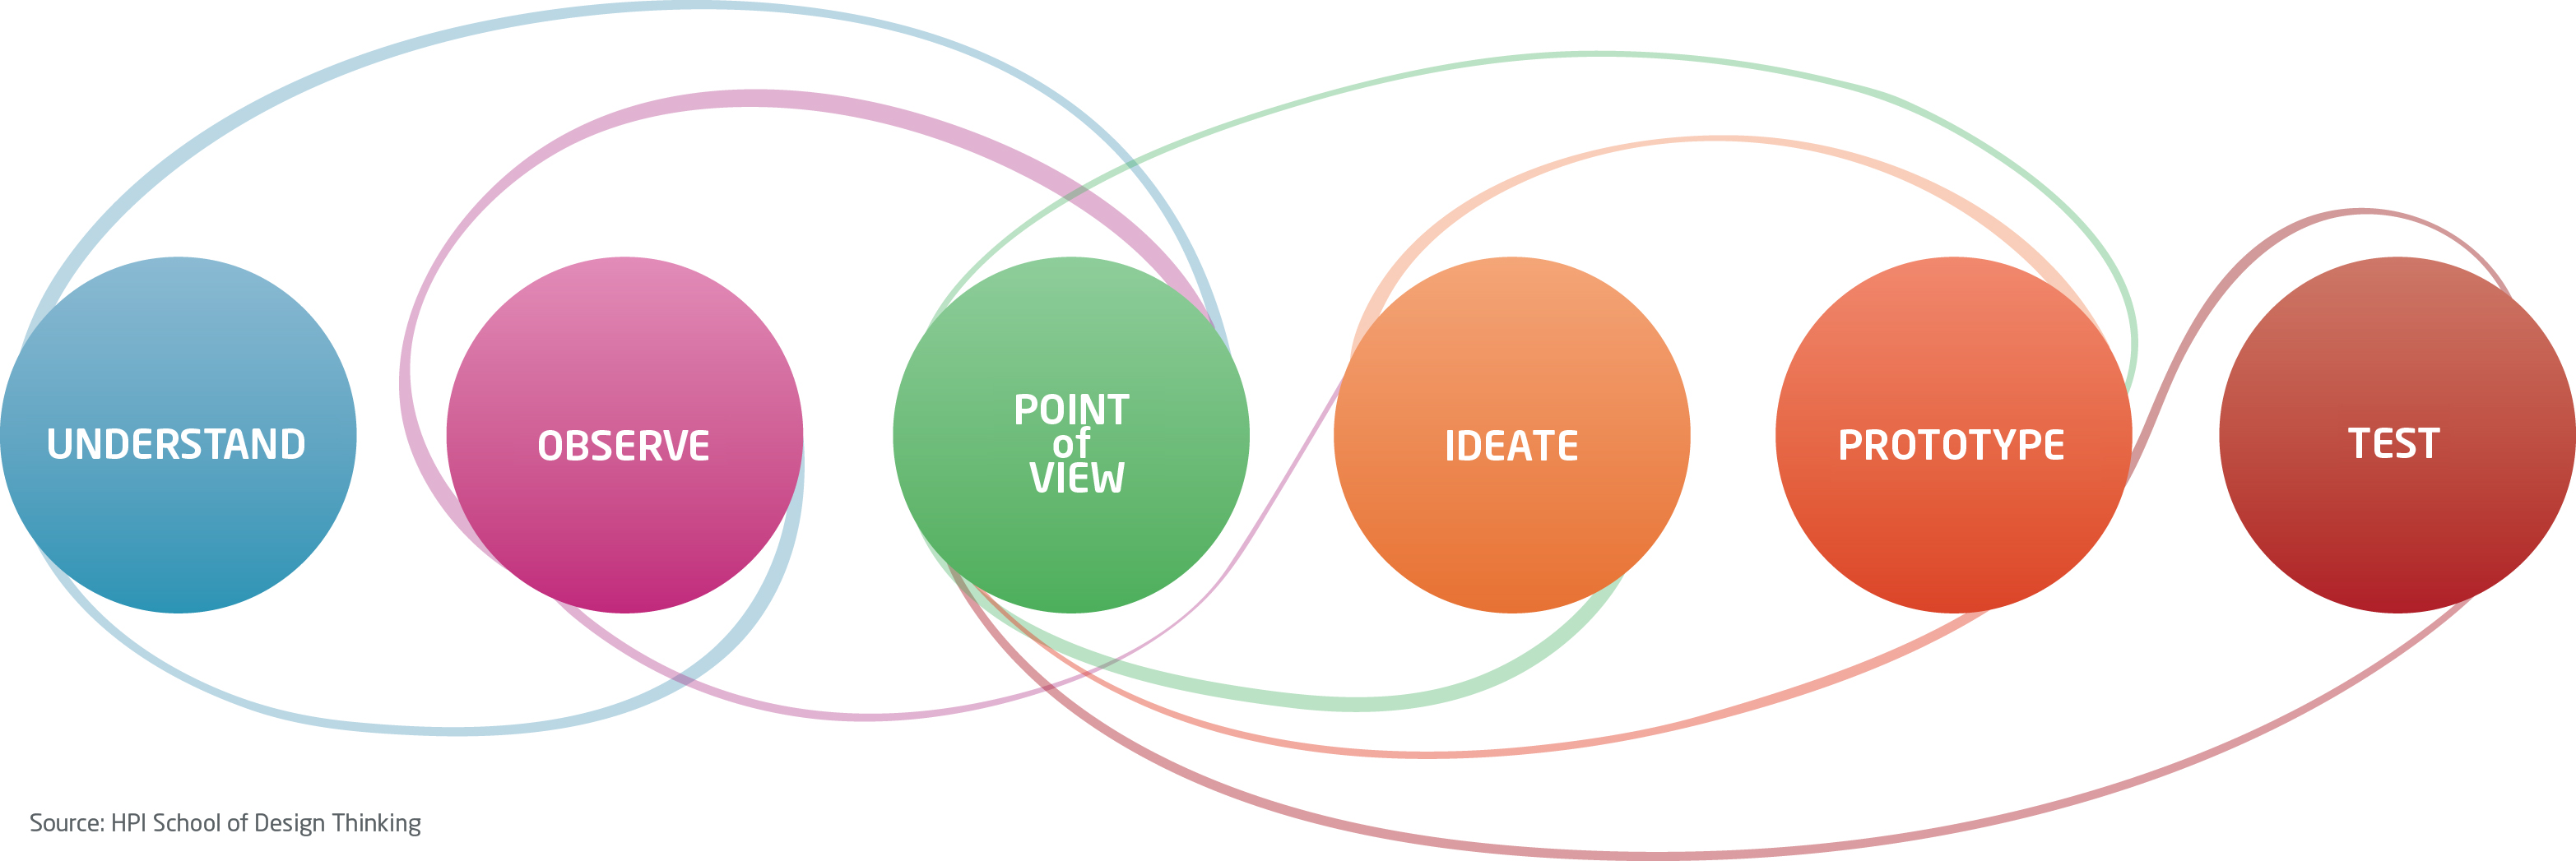
\includegraphics[width=\textwidth]{HPI_School_of_Design_Thinking_-_Prozess_en.jpg}
\caption{An overview of the phases in the Design Thinking process. Source: \cite{Plattner_2009}}
\label{fig:DT_phases}
\end{figure}

The projects usually deal with a problem posed by an industry partner. The Design Thinking method includes an iterative process which consists of several well-defined phases, shown in figure \ref{fig:DT_phases}. The phases guide the teams from basic understandings to the development of testable prototypes. The process is non-linear because the teams are encouraged to iterate. These cycles help to refine the prototypes based on actual user feedback. Throughout the process the students are being advised by teachers.
The D-School provides several team workspaces. A typical workspace consists of a set of whiteboards and a standing desk, which is large enough for the whole team to work on. The D-School considers open spaces to be important for the creative process, so the equipment is usually movable. Therefore, the spaces are hosted in large halls. The D-School also provides tools and materials for rapid prototyping.

There are several staff members at the D-School for coordinating and acquiring the student's projects. Key stakeholders for this thesis are the Head of D-School, the Program Manager, the Knowledge Manager and the Track Managers.

\section{Design process}
The Bachelor project also applied an iterative process, which is very similar to the one taught at the D-School. With this approach the project participants were able to benefit from the Design Thinking method while automatically learning about some of the needs of the D-School students.

\begin{figure}
\missingfigure{Prototype pictures}
\caption[Prototypes created during the first design iteration]{Prototypes created during the first design iteration: \textit{(a)} Doku-King: a gamification\footnotemark approach, where players earn points by documenting their work and validating the results of others. \textit{(b)} Doku-Board: a preformatted white board, where students create daily summaries of the most important insights or results. \textit{(c)} a rich-text-based editor, where students can summarize their results structured by the Design Thinking phases.}
\label{fig:First_prototypes}
\end{figure}

\footnotetext{Gamification is a trend that connects concepts of human-computer-interaction and game studies. \cite{Deterding_2011}}

During the project there have been several interviews with the relevant stakeholders. The group learned about the student's documentation efforts, especially commonly used methods and tools. Other stakeholders like teachers or D-School staff members have also been interviewed. Based on this information, the prototypes shown in figure \ref{fig:First_prototypes} were developed to enhance the documenting experience of the students. These prototypes were evaluated during user testing sessions.

\chapter{System Design}
In the second iteration a new prototype was designed which also addressed the need of the staff members to archive and categorize the projects for easy retrieval. This prototype is called ``Project Zoom". The following sections will highlight the most relevant use cases and requirements for this thesis.\footnote{The ``Software Requirements Specification"\cite{ReqSpec} covers the use cases and requirements in detail.}

\subsection{Use Cases}
Project Zoom addresses two main use cases, which were distilled from the insights gathered in the observation phases.

\begin{enumerate}
\item Student teams document their projects by organizing the digital documents they created in a visual manner.\\
\textsc{Prerequisite}: The students have all documents they created digitally available.\\
\textsc{Postcondition}: A visual knowledge graph is being created. \label{uc:organize}

\item D-School staff members get an overview of all projects. This overview enables access to the projects' classifications, related people and documentations.\\
\textsc{Prerequisite}: The projects were entered in a database (e.g. \textsc{Filemaker}\footnote{The D-School uses a \textsc{Filemaker} database to store projects and contacts. \url{http://www.filemaker.com/}, accessed 06/16/13}) and the students have documented their projects.\\
\textsc{Postcondition}: A visual representation of all projects is displayed. \label{uc:display}
\end{enumerate}

Beyond these two major use cases there are other relevant use cases.

\begin{enumerate}
\setcounter{enumi}{2}

\item The students add additional documents from their computers at home.\\
\textsc{Prerequisite}: The students have the documents digitally available.\\
\textsc{Postcondition}: The documents are included in the knowledge graph. \label{uc:fromhome}

\item Students, teachers and D-School staff members can retrieve states of the knowledge graph at different points in time.\\
\textsc{Prerequisite}: The students have documented their projects using the proposed tool.\\
\textsc{Postcondition}: A historical version of the knowledge graph is displayed.  \label{uc:versions}

\item Students can access the documents they saved using different commonly-used storage providers, e.g. \textsc{Box}\footnote{The D-School uses \textsc{Box} as a shared storage service. \url{https://www.box.com/}, accessed 06/16/13}.\\
\textsc{Prerequisite}: The students stored documents using the respective service.\\
\textsc{Postcondition}: Documents are offered for insertion in the knowledge graph.  \label{uc:storageproviders}

\item The Head of D-School and Program Manager show an overview of a customizable set of projects to potential industry partners using a mobile tablet device.\\
\textsc{Prerequisite}: The projects were entered in a database, e.g. \textsc{Filemaker}.\\
\textsc{Postcondition}: A visual representation of the projects is displayed. \label{uc:multiplatform}
\end{enumerate}

\subsection{Requirements}

To fulfill these use cases there are some technical requirements for designing and implementing Project Zoom. The following is a selection of relevant requirements.

\begin{enumerate}
\item The system's interface has to support multiple platforms, including the popular desktop operating systems and modern tablet devices. (use cases \ref{uc:fromhome}-\ref{uc:versions}) \label{req:multiplatform}
\item The system's interface has to be accessible from outside the D-School. (use case \ref{uc:fromhome}) \label{req:fromhome}
\item The systems has to support concurrent users accessing and modifying contents. \textit{Simplifying assumption}: Only one user is modifying one resource (e.g. a project's graph) at the same time. Multiple users may access different resources exclusively \todo{clear now?}. \label{req:concurrency}
\item The system connects to different data sources, e.g. \textsc{Box} and \textsc{Filemaker}, and makes the stored data available through its GUI. (use cases \ref{uc:organize},\ref{uc:storageproviders}) \label{req:storageprovider}
\item The system connects to the database the D-School uses to store projects and contacts. (use case \ref{uc:display}) \label{req:filemaker}
\end{enumerate}

\subsection{Design}
\label{sec:design}

Project Zoom is designed to apply the concept of semantic zooming. Semantic Zoom is part of the computer interface model \textsc{Pad} proposed by Perlin and Fox \cite{Perlin_1993}. This concept taps into the natural spatial thinking of users. Information is displayed on a large infinite two-dimensional canvas. Users browse around either by panning or zooming. There are different representations of the same pieces of information at different magnification levels. When zoomed out, documents are only represented by an icon or a title string. While zooming in, these abstract figures gradually resolve into the full representation of the respective documents. 

In Project Zoom there are three main zoom levels: An overview of all projects (\textbf{Overview view}), a detailed view of a project and its metadata (\textbf{Details view}), and a view containing a project's knowledge graph (\textbf{Process view}). Users can navigate from one view to the next by zooming in and out. This approach allows building one cohesive system, which hosts interfaces that are targeted at the specific needs of different stakeholders (see use cases \ref{uc:organize}-\ref{uc:storageproviders}). 

The main views themselves also support different zoom levels. Especially the Process view takes advantage of the zooming capabilities and displays the documents in the graph in different levels of detail. 
The Process view is an interactive graph that allows users to add documents onto the canvas and connect them with edges. The document nodes can then be annotate using the commenting feature or by drawing clusters (i.e. free form shapes) around them. These actions are exposed through context-sensitive menus. Also, the interactive graph features automatic layout capabilities, like collision prevention.

\subsection{Choosing a basic architecture}
In the design phase multiple architectures for Project Zoom have been evaluated. 

A \textbf{monolithic application} \footnote{Wikipedia, Monolithic application, \url{http://en.wikipedia.org/w/index.php?title=Monolithic_application&oldid=552899667}, accessed 06/17/13} is a self-contained system that can run on a single computer. The benefits are that the data is consistent for all users.  Also, the system is easy to set up because there is only one computer required for the system to work. This approach is well suited for applications that deal with independent datasets, which can be stored on one platform. Word processors are an example of monolithic applications. However, as use cases \ref{uc:fromhome} and \ref{uc:versions} as well as requirements \ref{req:multiplatform} and \ref{req:concurrency} require the data to be accessible on multiple platforms concurrently this architectural approach isn't suitable for Project Zoom.

The \textbf{peer-to-peer} \cite{Schollmeier_2001} architecture allows the distribution of data on multiple connected computers. Each node in the network is equally privileged and handles a subset of the data individually. Data consistency can be eventually achieved through replication from on neighbor node to another. This is a well-known database problem \cite{Gray_1996}. Access control can be integrated by using trusted computing technology \cite{Sandhu_2005}. Peer-to-peer architectures are usually applied when a centralized controlling instance is to be avoided. Bitcoin\footnote{Bitcoin, \url{http://bitcoin.org/}, accessed 06/25/13} is a popular peer-to-peer application. The ability of a node to function, especially when joining the network, depends on the availability of neighbor nodes. Because of the low number of users the availability of nodes might pose as an issue in Project Zoom. Also, implementing a peer-to-peer usually requires to build a native application which makes it harder to fulfill requirement \ref{req:multiplatform}.

The \textbf{client-server} \cite{Berson_1996} model is one of the most-used distributed architectures. One central computer acts as a server which stores the dataset and manages access control. Client computers can access and modify the resources on the server through a network interface. An example of a client-server application is the World Wide Web. Fundamentally, the server is a single point of failure \footnote{Wikipedia, Single point of failure, \url{http://en.wikipedia.org/w/index.php?title=Single_point_of_failure&oldid=555725127}, accessed 06/17/13}. However, there are methods to maximizing the availability \cite{Gray_1991} \cite{Colyer_2000}. This architecture is suitable for Project Zoom as it fulfills all the requirements, especially \ref{req:multiplatform}–\ref{req:concurrency}, and enables all the use cases.

A web-based client-server architecture is a system that uses an HTTP-Server \cite{RFC2616} and a browser application as client. Project Zoom incorporates this approach for several reasons:
\begin{itemize}
\item Using the client application of a web-based system only requires the installation of a web browser, which are wide-spread and usually preinstalled on the operating system. This makes it easy for students to modify the data from their computers at home (see: use case \ref{uc:fromhome}).
\item Developing native apps for mobile devices requires different technologies for each platform \cite{Charland_2011}. However, recent mobile devices are equipped with HTML5-capable \cite{W3C_HTML5} web browsers. Applications built using web technologies are likely to run on multiple mobile platforms (see: requirement \ref{req:multiplatform}).
\item Because of the standardization of the web technologies, emerging platforms will likely to support them as well.
\end{itemize}

Alternatives to a web-based client-server architecture are based on client applications that users have to install on their devices. Because the users of Project Zoom use multiple computing devices, this isn't a favorable approach, as the application has to be installed on each device separately. Also, users may not even be able to install the application on to the device due to imposed access restrictions.

\subsection{Architecture overview}

\begin{figure}
\missingfigure{Complete Architecture diagram}
\caption{Architecture overview of Project Zoom}
\label{fig:CompleteArchitectureDiagram}
\end{figure}

Figure \ref{fig:CompleteArchitectureDiagram} shows the system architecture of Project Zoom. The server implementation features an event-system that is fed by the data connectors and sets up the pipeline for thumbnail generation. The server also hosts the database model and handles user access control and authentication. Client and server are connected through a REST interface \cite{Fielding_2000}. The client application is built using an MVC pattern, which will be detailed in later chapters. 

\subsection{Project context}
There are six theses covering Project Zoom. Bocklisch \cite{Bocklisch_2013} describes the architecture of the server and the domain data model. Werkmeister \cite{Werkmeister_2013} details the connection of the data providers, e.g. \textsc{Box} and \textsc{Filemaker}, to the system. Bräunlein's thesis \cite{Braeunlein_2013} covers both the design and generation of document thumbnails for the Process View. Dieckhoff \cite{Dieckhoff_2013} details the automatic layouting capabilities of the interactive graphs. Herold \cite{Herold_2013} explains the context-sensitive actions that users can perform on the graph and its nodes and edges. This thesis is about the architecture of the client application.
    
    \chapter{Client Application Architecture}

\section{Overview}
The client application of Project Zoom is a web-based application. It can be run using an HTML5-capable web browser. The client application accesses the server's resources through a REST interface. The code is partitioned into several modules. An architectural pattern similar to Model-View-Controller (MVC) is applied.

\subsection{MV* pattern family}
The Model-View-Controller (MVC) pattern was first introduced by Reenskaug in 1979 \cite{Reenskaug_1979} and later published by Krasner et al. in 1988 \cite{Krasner_1988}. It was one of the first approaches to separate business and presentation logic code within a software project.

\begin{figure}
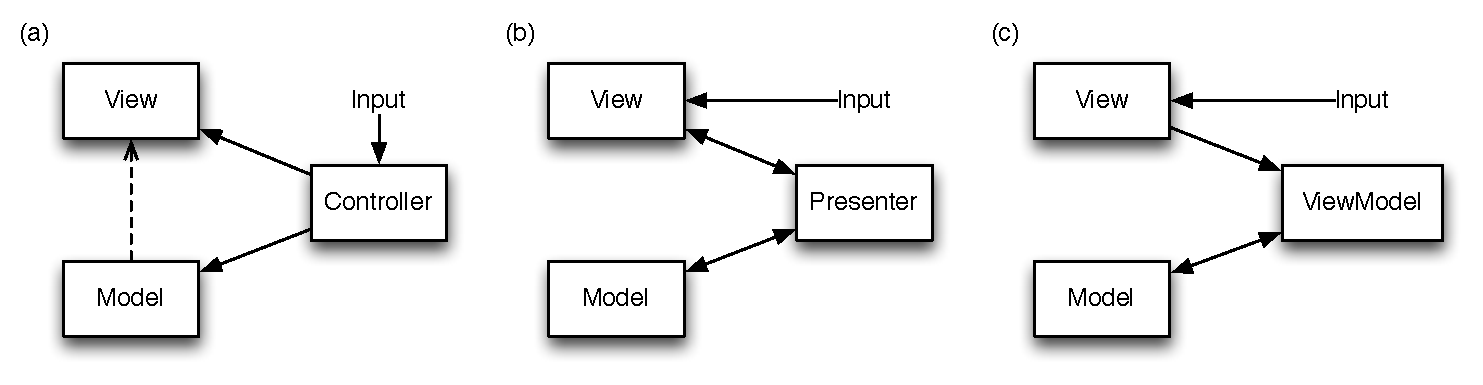
\includegraphics[width=\textwidth]{mvc-mvp-mvvm.pdf}
\caption[Diagrams of Model-View-Controller, Model-View-Presenter and Model-View-ViewModel]{\textit{(a)} Model-View-Controller \textit{(b)} Model-View-Presenter \textit{(c)} Model-View-ViewModel}
\label{fig:MV}
\end{figure}

A \textbf{Model} is an active representation of the data in the system. It usually encapsulates methods for fetching, persisting and transforming the data. It also emits events upon data changes that Controllers and Views can listen to. The Model itself is agnostic of any particular user interface. A \textbf{View} encapsulates all the code required to display a user interface with the data from the Model. A \textbf{Controller} is responsible for updating the Model when a user manipulates the View. \cite{Krasner_1988} \cite{Gamma_1994}

Since its introduction in the 1980s the MVC has mutated to accommodate modern technologies. The architectural patterns MVC, Model-View-Presenter (MVP) and Model-View-ViewModel (MVVM) as shown in figure \ref{fig:MV} a–c are commonly referred to as the MV* pattern family \cite{Osmani_2012}. As the separation of business and presentation logic MV* patterns are widely used in the development of web applications \cite{Takada_2012}.

Model-View-Presenter (MVP) is derived from MVC to achieve a complete separation between Model and View. Whereas in MVC the View depends on the Model, in MVP the View is agnostic to a specific Model and can be reused for different Models. The Presenter replaces the Controller and has the responsibility to connect the interfaces of Model and View. 

Model-View-ViewModel (MVVM) is based on the concepts of MVP. However, the Presenter is replaced by a ViewModel, which contains a subset of the Model as well as additional state and methods. The ViewModel and the View communicate through data-binding\footnote{Data-binding is a technique where properties of a Model can be assigned to user interface components in a way that changes from either one are reflected to the other. \cite{Bent_2004}} and events. Since Model and View are separated the ViewModel connects both and contains logic in state-change and event handlers.

MVP and MVVM are commonly used in scenarios in which it is important to have user interface components that are of general-purpose and have to be reused in several different locations. Such applications are usually enterprise or consumer applications with a large number of Views. MVC is a more lightweight approach, which is well suited for applications with a smaller number of Views and conceptual tight coupling between presentation and data. \cite{Osmani_2012}

The client application of Project Zoom only has a few Views, as described in section \ref{sec:design}. The interactive graph (cf. use case \ref{uc:organize} and \ref{uc:versions}) is a very close representation of the respective Model. Besides, it has to be custom developed, as there are no applicable standard components available. Based on these observations the MVC architecture has been selected for the client application of Project Zoom. Figure \ref{fig:arch} shows the implemented architecture. The components shown are detailed in later sections.

\begin{figure}
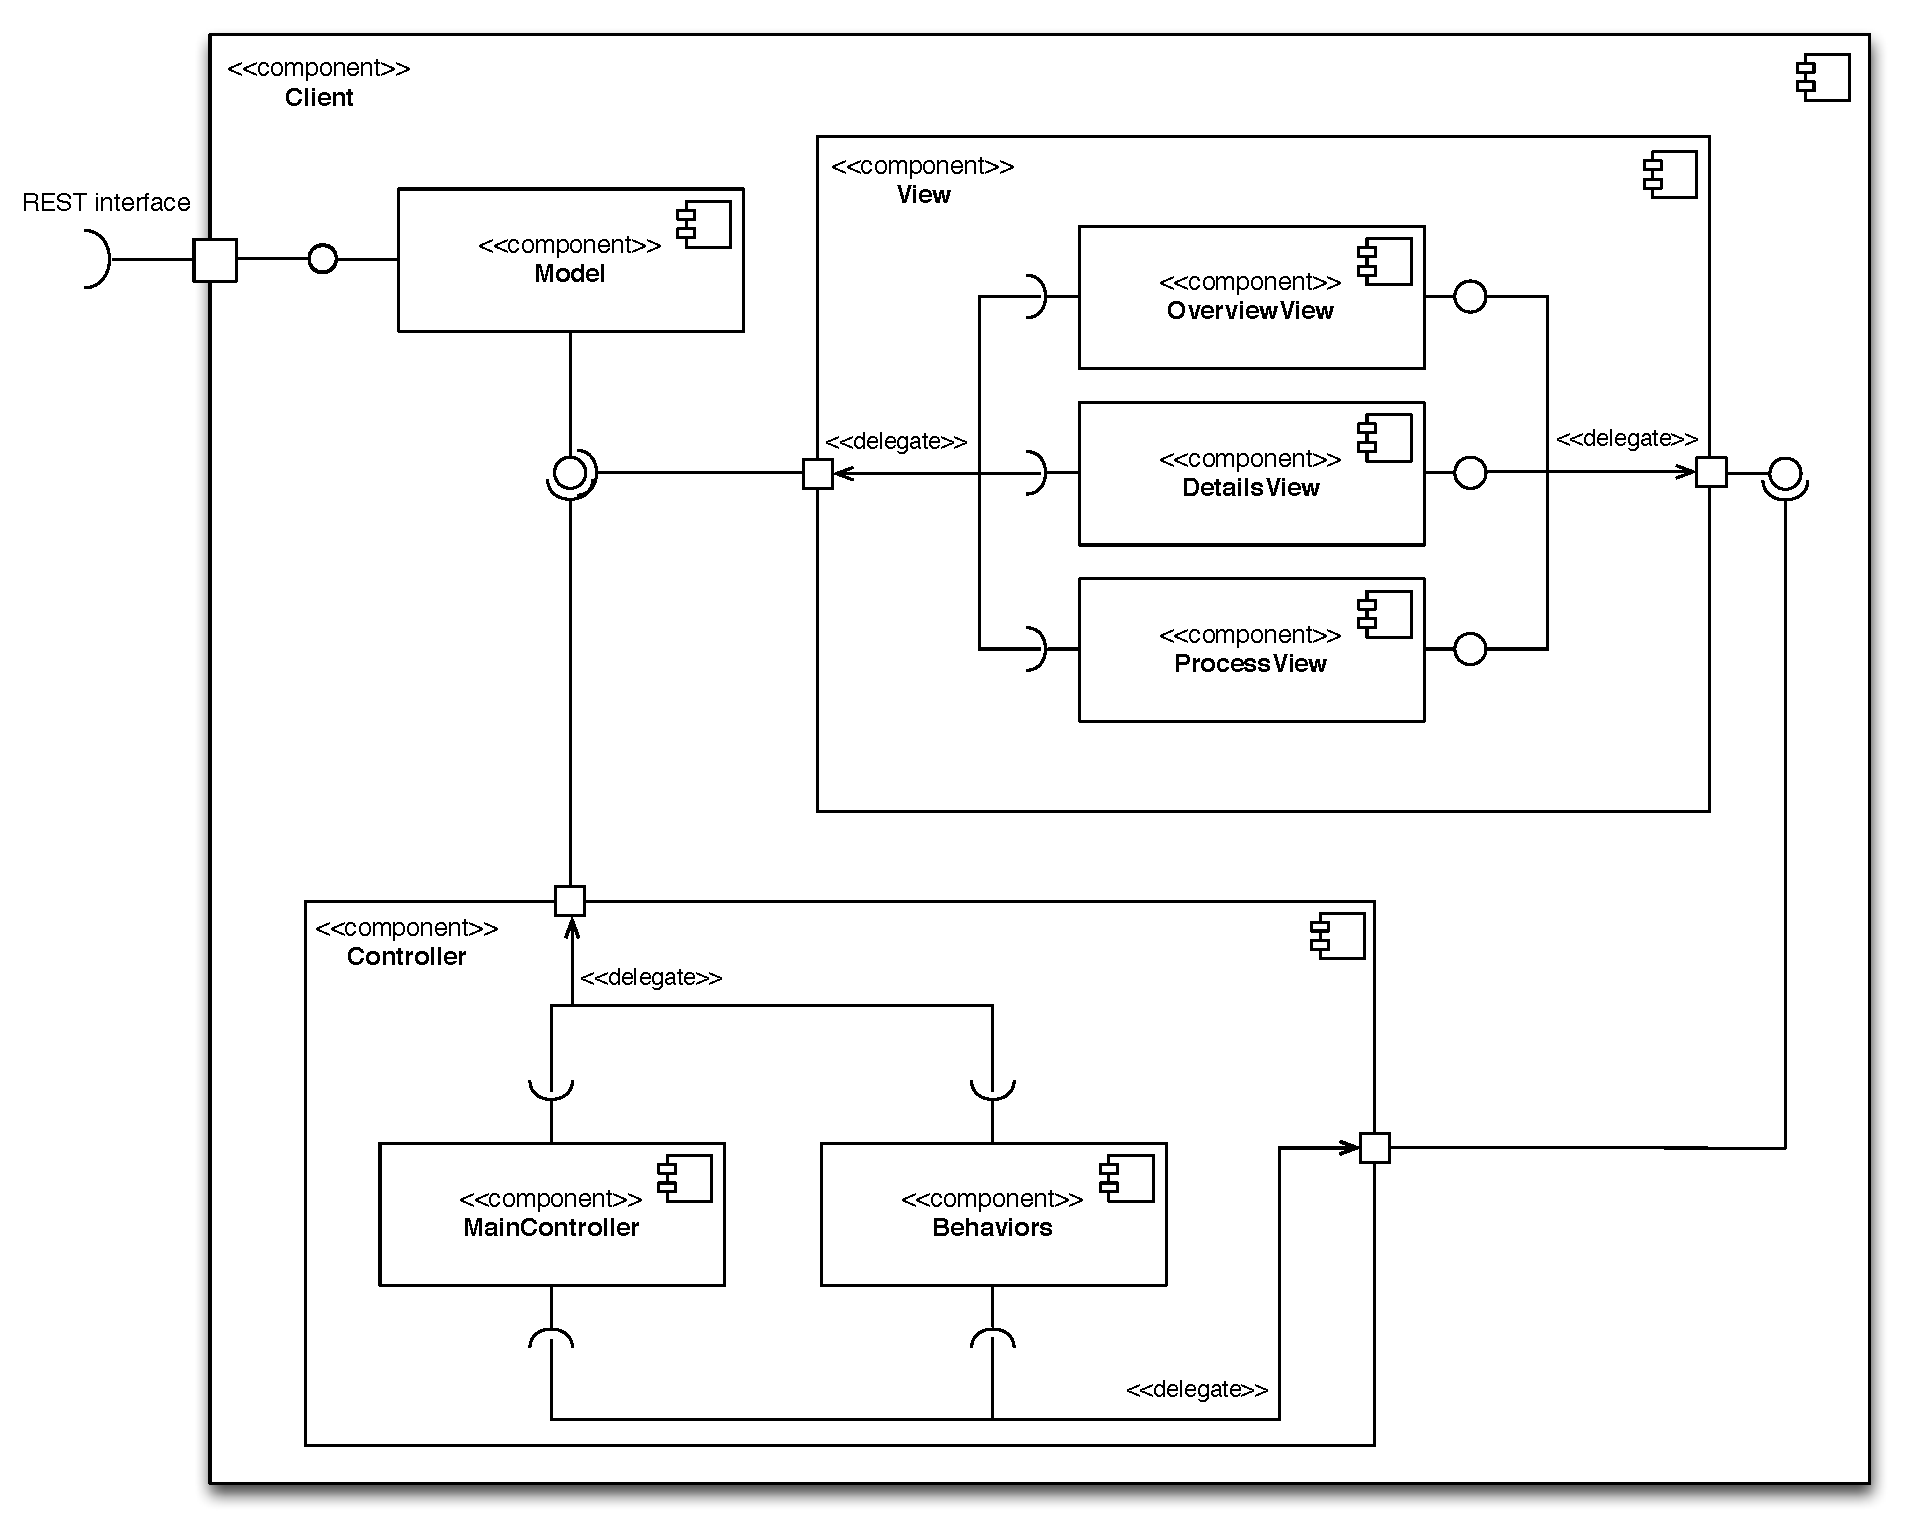
\includegraphics[width=\textwidth]{clientarchitecture2.pdf}
\caption{Diagram of the client application architecture.}
\label{fig:arch}
\end{figure}


\subsection{Event-driven programming}
\label{sec:eventbased}

Users expect computer systems to respond quickly. This is especially true for web applications \cite{Selvidge_1999}. In any case users expect the interface to be non-blocking when the system is performing long running tasks \cite{Nielsen_1994}.  In web applications this is achieved by asynchronous APIs for tasks like requesting data from the server \footnote{XMLHttpRequest, \url{http://www.w3.org/TR/XMLHttpRequest/}, accessed 06/19/13} or waiting for user input \footnote{Document Object Model (DOM) Events, \url{http://www.w3.org/TR/DOM-Level-3-Events/}, accessed 06/19/13}. An event-driven system is a popular solution for dealing with asynchronous code execution \cite{Michelson_2006}. 

\textbf{Events} are messages sent between components in a system. The receiver has to subscribe to a type of events, which senders then eventually publish (cf. Observer pattern \cite{Gamma_1994}). There are two categories of events:
\begin{itemize}
\item Global events are only identified by their names and can be received by any object in the system.
\item Object specific events are identified by both their names and sender objects. Receivers need to have a reference to the sending object when subscribing to this kind of events.
\end{itemize}

Event-driven programming is a concept where components of a system heavily communicate via events. Particularly, data changes and user actions are propagated using events. Taking an event-driven approach leads to looser coupling between components and consequently, to better testable and maintainable code \cite{Faison_2011}.

Requesting data from the server (cf. use case \ref{uc:fromhome}), waiting for user inputs and listening to data synchronization messages (cf. requirement \ref{req:concurrency}) are asynchronous tasks that the Project Zoom client performs. Using an event-driven architecture allows the system to pass data streams efficiently through the system.

\subsection{Synchronization}
As a collaborative web application, Project Zoom allows multiple users to access and manipulate shared resources (cf. requirement \ref{req:concurrency}). There are four popular approaches for dealing with synchronization issues in distributed systems: Locking, Operational Transformation, three-way merges and Differential Synchronization \cite{Fraser_2009}.

\begin{figure}[!h]
\begin{center}
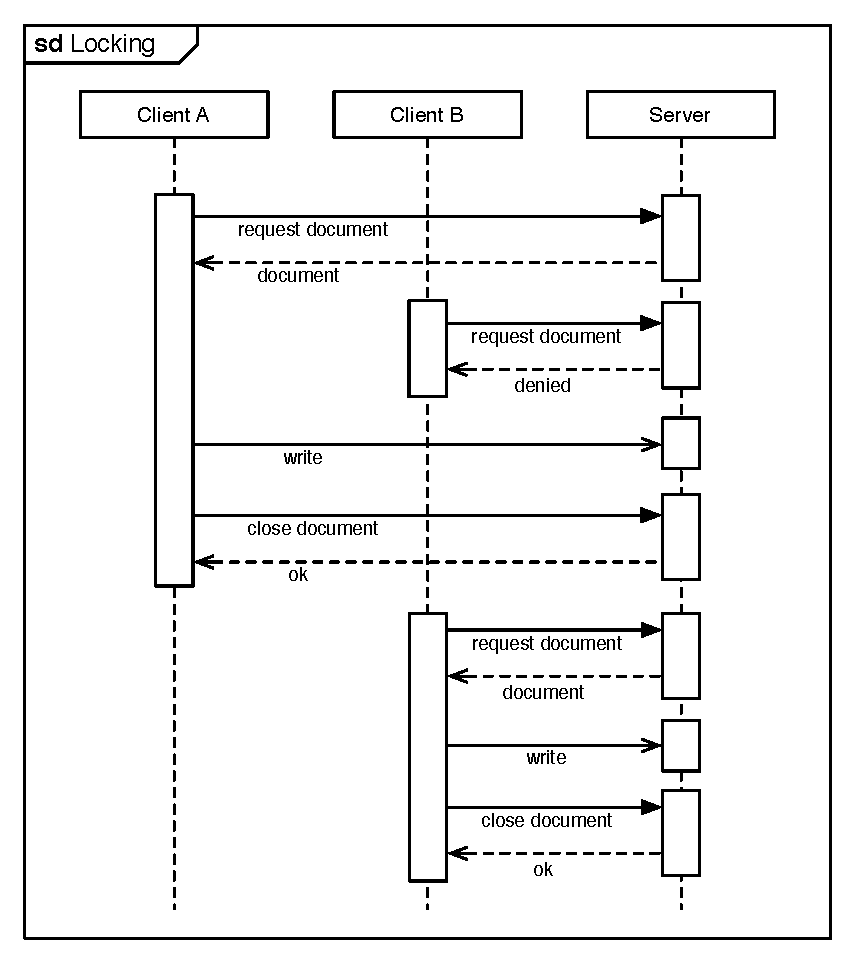
\includegraphics[width=0.5\textwidth]{locking_seq.pdf}
\caption{Sequence diagram of synchronization with locking}
\label{fig:locking}
\end{center}
\end{figure}

\textbf{Locking} is a mechanism to enforce mutual exclusion and is a standard solution for synchronization \cite{Dijkstra_1965}. Figure \ref{fig:locking} outlines how locking ensures consistency as only one user has access to the resource at a time. Due to its ensured consistency locking is implemented in a variety of applications, e.g. ACID\footnote{Atomicity, Consistency, Isolation and Durability (ACID) are a set of properties that database transactions guarantee. \cite{Gray_1981}}-compliant database systems, office applications\footnote{File locking in Microsoft Word, \url{http://support.microsoft.com/default.aspx?scid=kb;EN-US;176313}, accessed 06/25/13} and document-collaboration software\footnote{MediaWiki Documentation: LockManager, \url{https://doc.wikimedia.org/mediawiki-core/master/php/html/classLockManager.html}, accessed 06/25/13}. As real-time collaboration\footnote{Real-time collaboration is a mechanism where the changes to a document on a client are immediately propagated to the other clients. Because of network-latency, the real-time property is in this context not as narrow as in the fields of operating systems or computer graphics. \cite{Sun_2002}} systems require concurrent access to shared resources, locking is not suitable for this class of systems.

\begin{figure}[!h]
\begin{center}
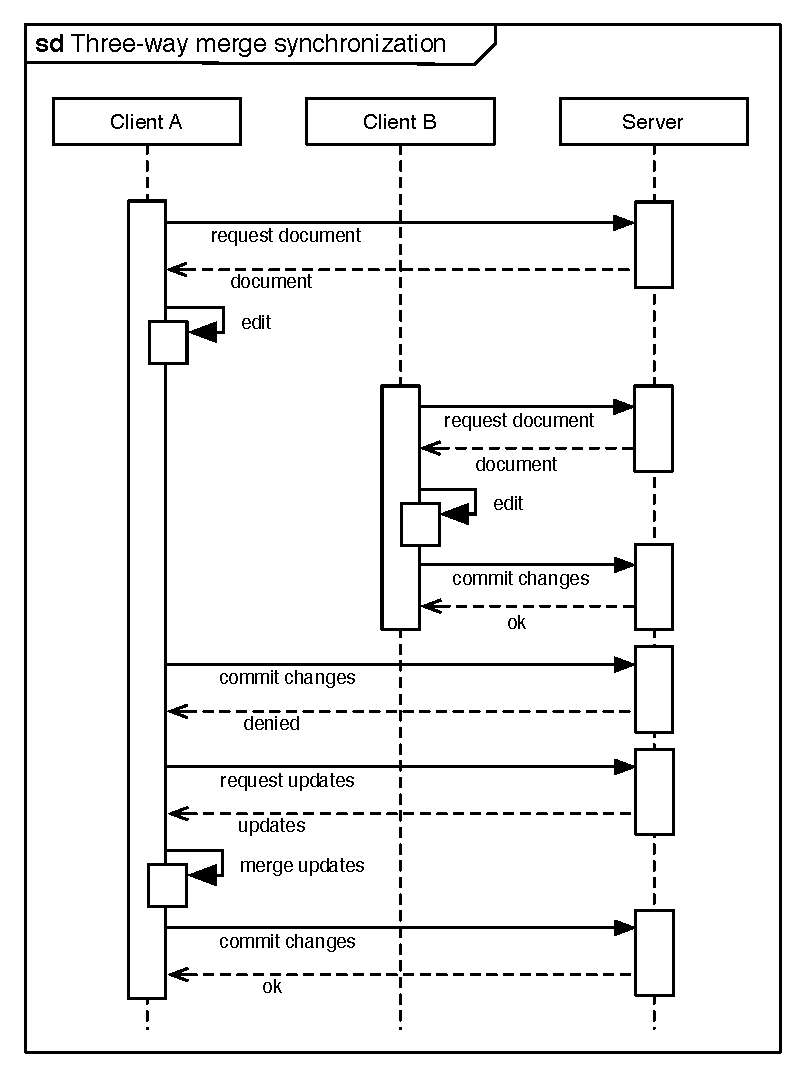
\includegraphics[width=0.5\textwidth]{threeway_seq.pdf}
\caption{Sequence diagram of three-way merge synchronization}
\label{fig:threeway}
\end{center}
\end{figure}

The \textbf{three-way merge} is a synchronization approach that has been implemented in some revision control systems \cite{Pilato_2008}. As shown in figure \ref{fig:threeway}, the clients hold a local version of a document and make edits to it individually. When synchronizing these changes, the client first requests updates from the server and merges them locally. Then, the synchronized data is sent back to the server. A system using the three-way merge approach is not guaranteed to be consistent as synchronization is only triggered when a client publishes an edit. This edit is not automatically propagated to other collaborating clients. Therefore, this approach is not suitable for real-time collaboration systems either.

\begin{figure}[!h]
\begin{center}
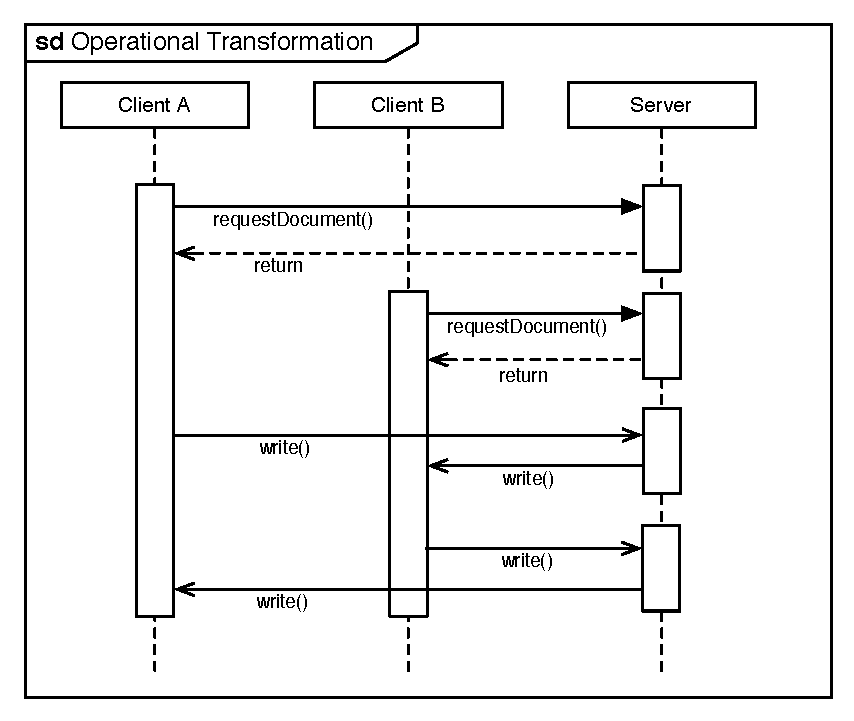
\includegraphics[width=0.5\textwidth]{ot_seq.pdf}
\caption{Sequence diagram of Operational Transformation}

\label{fig:optr}
\end{center}
\end{figure}


\textbf{Operational Transformation} (OT) is a class of algorithms that use event-passing for synchronization \cite{Ellis_1989}. Figure \ref{fig:optr} shows the interaction scheme of OT. All user actions on the document are captured in form of change events and then sent to the collaborating clients. These change instructions are commonly known as patches. \textit{Eventual consistency}\footnote{Eventual consistency describes that all accesses to a resource yield the same result when there have been no writes in a particular time span. \cite{Gustavsson_2002}} can be achieved through different models \cite{Sun_1998} \cite{Li_2004} \cite{Li_2005}. Google Docs\footnote{Google Docs, \url{https://docs.google.com/}, accessed 06/25/13} is a popular example application that uses OT.

\textbf{Differential Synchronization} is very similar to OT \cite{Fraser_2009}. However, instead of capturing all changes as they happen, the change instructions are distilled by comparing two snapshots of the document. This approach is preferred when capturing all the user edits is a practical challenge.

Even though concurrent editing of the same document is not a requirement, concurrent read access is (cf. requirement \ref{req:concurrency}). Using automatic updates instead of manual ones greatly enhances the user experience. Both Operational Transformation and Differential Synchronization support real-time collaboration. Therefore, they are the best-suited approaches for Project Zoom. However, as highlighted in section \ref{sec:eventbased}, an event-driven architecture has a lot of advantages, Operational Transformation is better fitting.

\subsection{Technology}
Since Project Zoom is a web application, the client code needs to be written in JavaScript\footnote{JavaScript is a scripting language that was designed for the use in web browsers and was standardized under the name ECMAScript \url{http://www.ecma-international.org/publications/files/ECMA-ST/Ecma-262.pdf}.}. The presentation layer is built using the standard HTML\footnote{Hypertext Markup Language, \url{http://www.w3.org/TR/html5/}, accessed 06/19/13} and CSS\footnote{Cascading Style Sheets, \url{http://www.w3.org/TR/css-2010/}, accessed 06/19/13} technologies. The interactive graph relies on SVG\footnote{Scalable Vector Graphics, \url{http://www.w3.org/TR/SVG/}, accessed 06/19/13} because of its unique zooming and hit-test\footnote{Hit-testing is a technique to determine which user interface element intersects with the user's cursor \cite{Foley_1995}.} capabilities. The d3\footnote{Data-Driven Documents, \url{http://d3js.org/}, accessed 06/19/13} library is used to manipulate the SVG document.

\section{Model}

The Model is the component that is responsible for fetching the data from the server, listening to changes and passing changes back to the server. Figure \ref{fig:modelinteraction} shows how changes to the data in the Model are propagated throughout the system. This section covers the techniques the client applies to handle the domain data on an abstract level. Bocklisch's thesis describes the actual domain data model in detail \cite{Bocklisch_2013}.


\begin{figure}
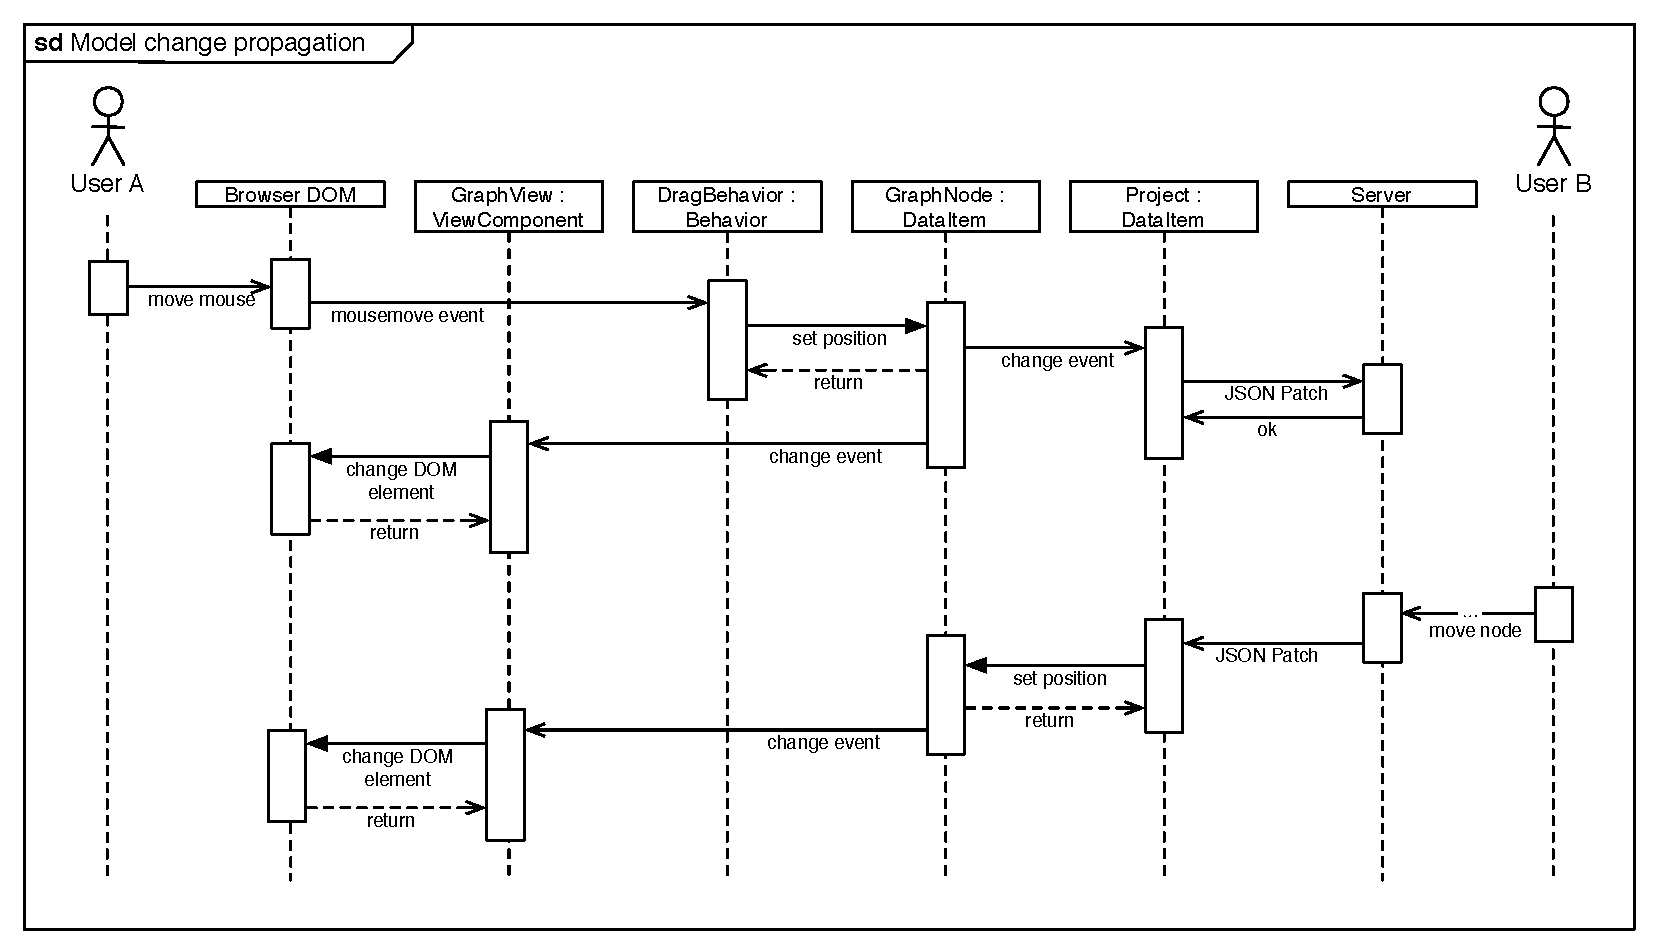
\includegraphics[width=\textwidth]{mvcinteraction.pdf}
\caption{Sequence diagram of an example event-driven change propagation.}
\label{fig:modelinteraction}
\end{figure}



\subsection{Representing the data in the client application}

The data is represented through two container classes that wrap around the native objects of Ja\-va\-Script: \texttt{DataItem} and \texttt{DataCollection}. Both classes extend the native objects with getter and setter methods for accessing and manipulating the respective properties or items. Using getters and setters is a popular technique of tracking changes in the data and emitting corresponding events \cite{Osmani_2013}. An alternative approach to container classes would be the \texttt{Object.observe} API\footnote{Harmony Observe (proposed standard), \url{http://wiki.ecmascript.org/doku.php?id=harmony:observe}, accessed 06/28/13} which has yet to be standardized \cite{Waldron_2012}.

The container classes can be used to build hierarchical tree structures. In such a structure, property changes of child objects are then propagated to their ancestor objects. In addition, nested properties can be accessed through the parent's \texttt{get} method using the JSON Pointer \footnote{RFC 6901, JavaScript Object Notation (JSON) Pointer, \url{http://tools.ietf.org/html/rfc6901}, accessed 06/20/13} syntax.

Both container classes provide methods for fetching data from the server. For that they use the XMLHttpRequest\footnote{XMLHttpRequest, \url{http://www.w3.org/TR/XMLHttpRequest/}, accessed 06/30/13} API of the browser. This technique is commonly referred to as Asynchronous JavaScript and XML (AJAX) \cite{Garrett_2005}. There is also support for \textit{lazy loading}\footnote{Lazy loading is a technique where data is only loaded once it is required, instead of loading it upon initialization. \cite{Fowler_2002}} of properties or subtrees. 


\subsection{Connecting to the server's REST interface}

\begin{figure}
\centering
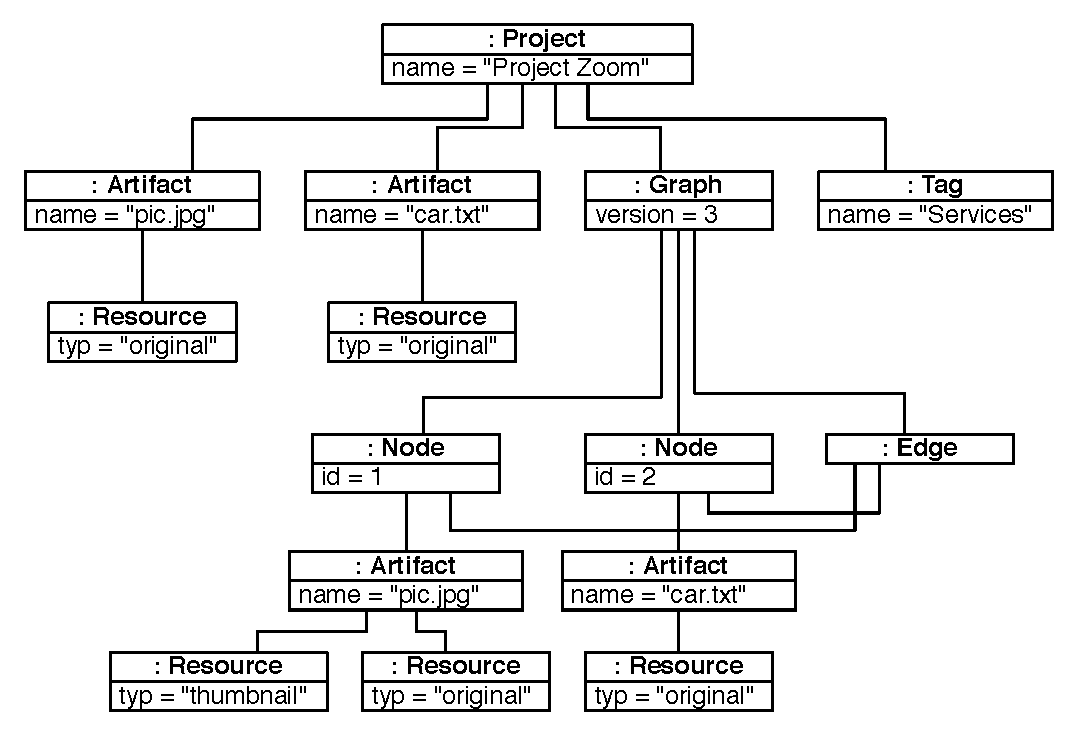
\includegraphics[width=0.7\textwidth]{object.pdf}
\caption{Object diagram of an example data structure.}
\label{fig:projectstruc}
\end{figure}

The server provides the data through a REST interface. Representational State Transfer (REST) is an architectural style on top of HTTP where resources are accessible through non-mutable URLs and are accessed and manipulated through the HTTP methods instead of custom URLs. \cite{Fielding_2000} 

The REST interface for Project Zoom relies on the JSON\footnote{RFC 4627,  The application/json Media Type for JavaScript Object Notation (JSON), \url{http://tools.ietf.org/html/rfc4627}, accessed 06/20/13} format for data exchange. As JSON is based on a subset of JavaScript, is very easy to parse and create JSON documents through native APIs. The full specification of the project's REST interface is attached in the Appendix \ref{appendix:REST}.

Upon initialization the Model requests the \texttt{projects} and \texttt{tags} collections from the server. This is useful because all business logic depends on these data collections. Lazy loading would increase page-loading time even further. As shown in figure \ref{fig:projectstruc} a project object is one of the root data structures in the system.


\subsection{Synchronizing changes with the server}

Changes to the server are transmitted using a patch-based format. Patches are documents that describe changes between two versions of a document. In many scenarios, patches have a substantially smaller footprint than their referenced document. Therefore, they are faster to send over a network. Furthermore, applying patches instead of replacing whole documents is less likely to cause consistency errors \cite{Ellis_1989}. Patches are also a key concept in Operational Transformation, which has been employed to support real-time collaboration.

Project Zoom uses the recently introduced JSON Patch standard \cite{RFC6902}. JSON Patch is a format for describing a list of mutations in an existing JSON document. A mutation entry contains an operation identifier, e.g. \texttt{add}, \texttt{remove} or \texttt{replace}, as well as a property address using the JSON Pointer syntax and a new value. Appendix \ref{appendix:JSONpatch} shows an example of a JSON patch applied to a JSON document. 
An accumulator object generates the JSON patches. It connects to a \texttt{DataItem} object and listens to the change events. As \texttt{DataItem}s propagate change events from their child nodes, the accumulator can be attached to any node and will receive the change events from the complete subtree. For each change the accumulator appends a new patch entry to a list buffer, which will eventually be sent to the server.

For some user actions, e.g. dragging an element across the canvas, the number of patch entries can grow very fast. To minimize the transportation footprint of the patches, the accumulator provides a method for compacting patches by reducing the amount of redundant entries in the patch. The proposed algorithm is shown in listing \ref{lst:patchcompact} and has a time complexity of $\mathcal O(n^2)$. Compacted patches are then sent to the server using the HTTP \texttt{PATCH} method.

\begin{figure}
\begin{lstlisting}[language=pseudo,caption={Pseudo code for compacting a chronologically ordered list of JSON patches},label={lst:patchcompact}]
foreach patch1, i in patches
  # patch1.item is the object that is referenced by patch1.path
  
  if patch1 is marked as overridden
    remove patch1
  
  foreach patch2, j in entries where i > j
    if patch2 removes patch1.item or any parent of patch1.item
      remove patch1
      mark patch2 as overridden
      
    else if patch2 replaces patch1.item or any parent of patch1.item
      remove patch2
     
    else if patch2 replaces or removes a child of patch1.item
      merge patch2 into patch1
      mark patch2 as overridden
\end{lstlisting}
\end{figure}

The client is designed to listen to changes sent from the server. For that the client opens a WebSocket\footnote{WebSocket, \url{http://tools.ietf.org/html/rfc6455}, \url{http://www.w3.org/TR/2009/WD-websockets-20091222/}, both accessed 06/23/13} connection. The server sends JSON patches with an accompanying resource identifier, which get applied to the data structure in the client. Because of the event-driven architecture of the client, these changes will be propagated to the View immediately. As concurrent editing of a single resource (e.g. an interactive graph) is not a requirement (cf. requirement \ref{req:concurrency}), conflicting edits will be rejected by the server.

\section{View}

The View is responsible for rendering the data to the user interface. It is build from a set of components that bind to the data from the Model.

\subsection{Component interface}

\begin{wrapfigure}{R}{0.3\textwidth}
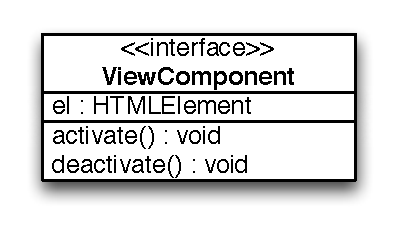
\includegraphics[width=0.3\textwidth]{viewinterface.pdf}
\caption{Class diagram of the View component interface}
\label{fig:viewinterface}
\end{wrapfigure}

The View is assembled by a hierarchical structure of View component instances. These instances share a common interface as shown in figure \ref{fig:viewinterface}. The View objects are responsible for controlling one element in the Document Object Model (DOM), which is referenced through the attribute \texttt{el}. At this stage the View component is not interactive yet. The method \texttt{activate} enables interactivity, by attaching event handlers to the DOM. \texttt{deactivate} then removes these event handlers, making the View component non-interactive again. This approach allows other components to control which View components are currently active. Consequently, parent components are responsible for activating and deactivating their children. The View components do not attach their element to the DOM themselves.

\subsection{Data integration}

Upon initialization View components are assigned with a \texttt{DataItem} or a \texttt{DataCollection}. The contained data is then used to render the user interface. Views tap into the event system and listen to changes from the Model to update accordingly. For example, when a user moves the cursor across the canvas to drag a graph node, the \texttt{position} property of the node is being altered by a Controller (cf. section \ref{sec:behavior}). This change is propagated to the View, which then renders the node at its new position. Server-sent changes are handled in the very same way. So, the View is agnostic to where the event originated.

\subsection{Architecture}

\begin{figure}
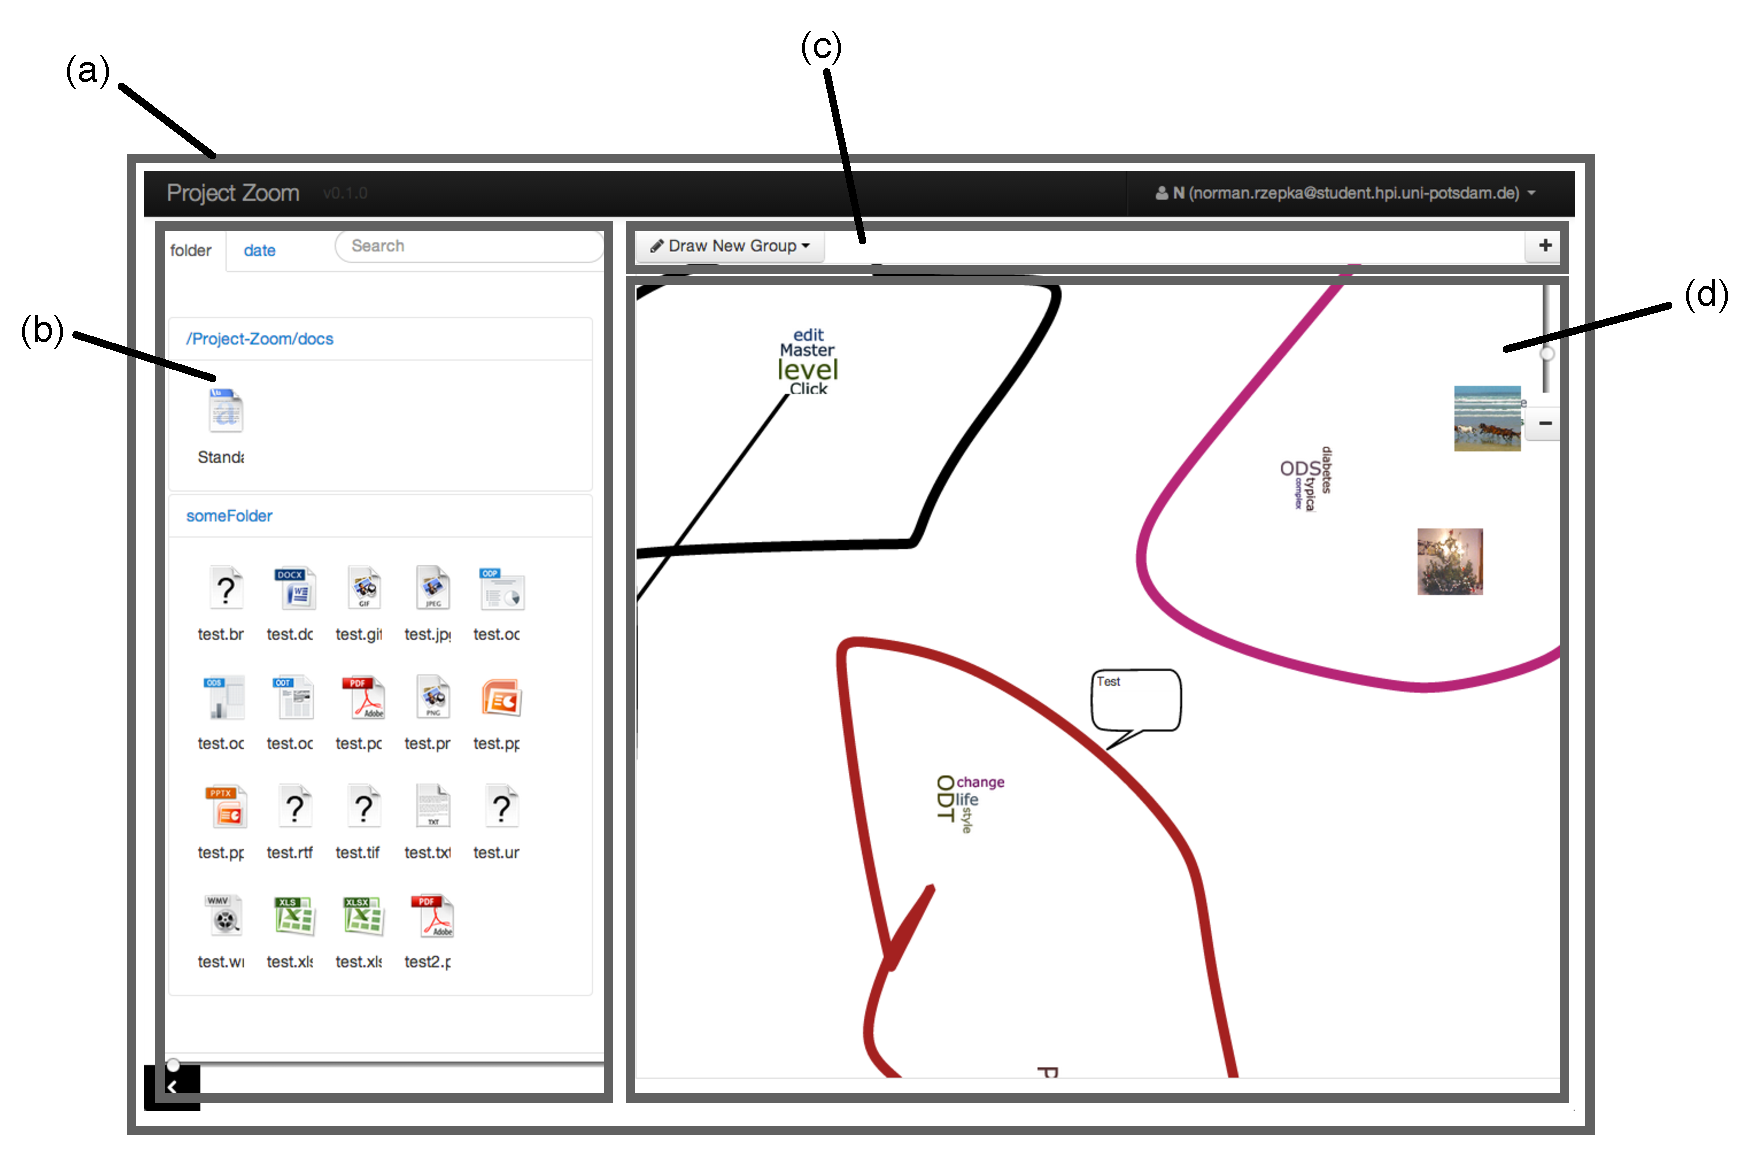
\includegraphics[width=\textwidth]{viewlayout.pdf}
\caption[Screenshot of the Process View with component annotations]{Screenshot of the Process View with component annotations: \textit{(a)} ProcessView, \textit{(b)} ArtifactFinder, \textit{(c)} Toolbar, \textit{(d)} Graph}
\label{fig:viewlayout}
\end{figure}

There are three main Views: Overview View, Details View and Process View (cf. section \ref{sec:design}). As shown in figure \ref{fig:arch} these are represented by three hierarchical View component structures. Figure \ref{fig:viewlayout} is an example of how the individual components have distributed responsibilities across the user interface.

\section{Controller}

The Controller components handle user interactions and manipulate the data in the Model as well as the Views.

\subsection{Main controller}
In Project Zoom, zooming is the main method for navigating from one View to another (cf. section \ref{sec:design}). The main Controller handles this zoom-based behavior. For that the domain of zoom levels is split into several subranges as shown in figure \ref{fig:zoomtable}. The controller enforces states of the main Views in each subrange as described.

The Controller works with the global range of zoom levels. This global zoom level is decoupled from the zoom level that the individual Views work with. Because of this it is easier to alter the parameters in the controller while maintaining the assumptions in the View components and vice versa. The controller converts the global zoom level into the specific levels using pluggable functions.

\begin{figure}
\begin{center}
\begin{tabular}{|c|c|c|c|}
\hline
& Overview View & Details View & Process View \\ \hline
0-9 & active & - & - \\
10-19 & transition-out & transition-in & - \\
20-29 & - & active & - \\
30-39 & - & transition-out & transition-in \\
40-150 & - & - & active \\ \hline
\end{tabular}
\end{center}
\caption{Zoom level configurations}
\label{fig:zoomtable}
\end{figure}

\begin{wrapfigure}{R}{0.3\textwidth}
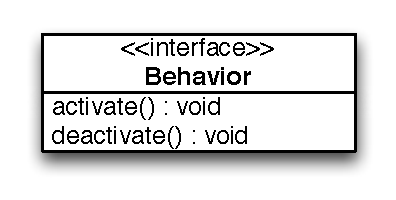
\includegraphics[width=0.3\textwidth]{behaviorinterface.pdf}
\caption{Class diagram of the Behavior interface}
\label{fig:behaviorinterface}
\end{wrapfigure}

\subsection{Behavior controllers}
\label{sec:behavior}

In addition to the main controller there are several other controllers that encapsulate a particular behavior in one of the main views, e.g. dragging nodes, drawing clusters or commenting. These behaviors share an interface as shown in figure \ref{fig:behaviorinterface}, which is similar to the interface of the View components . Again, the \texttt{activate} and \texttt{deactivate} methods enable or disable the interactivity provided by the respective behavior. Behaviors operate independently of each other and only communicate via events. For example, the deletion behavior emits an event whenever a node has been removed from the graph. The selection behavior recognizes this event and eliminates any references it had to that node. This loosely coupling makes it easy to extend the functionality of the application by adding custom behaviors. Behaviors alter the data in the Model. Because of the event-driven architecture these alterations are propagated to update the View and sent to the server for persistence.


    
    \chapter{Evaluation and Implementation}

\section{Use cases and requirements revisited}

This section explains how the proposed architecture of Project Zoom enables the use cases and fulfills the requirements that were previously established.

\begin{figure}
\begin{center}
\missingfigure{Use case 1 figure}
\caption{Sequence diagram for use case 1.}
\label{fig:evaluc1}
\end{center}
\end{figure}

\paragraph{\ref{uc:organize}} Figure \ref{fig:evaluc1} shows how files are pulled from a storage provider by the server\footnote{Werkmeister covers how the data is pulled from different kinds of storage providers, e.g. \textsc{Box} and \textsc{Filemaker}. \cite{Werkmeister_2013}} and sent to the client. Because of the implemented dragging behavior, a user is able to add these documents as a node to the visual graph. Using context-sensitive actions these node may be connected to others or annotated in different ways \cite{Herold_2013}. 

\begin{figure}
\begin{center}
\missingfigure{Use case 2 figure}
\caption{Sequence diagram for use case 2.}
\label{fig:evaluc2}
\end{center}
\end{figure}

\paragraph{\ref{uc:display}} The D-School uses a \textsc{Filemaker}\footnote{Filemaker, \url{http://www.filemaker.com/}, accessed 06/16/13} database to store projects. The server polls that database. The client can then access them through a REST interface and display them in a user interface. This interaction is outlined in figure \ref{fig:evaluc2}.

\paragraph{\ref{uc:fromhome}} Project Zoom is designed using a web-based client-server architecture. The server software is capable of handling requests from clients over a network connection. If the software is deployed on a public server, the application will be reachable from any internet-connected computer. Use case \ref{uc:fromhome} requires the users to have an installation of a HTML5-capable browser to access the application. Such web browsers are very popular and likely to be already preinstalled on the user's computer.

\paragraph{\ref{uc:versions}} When a graph in Project Zoom has been edited, it is automatically stored shortly afterwards in the server's database. Every version of a particular graph is kept in the database for later retrieval \cite{Bocklisch_2013}. The server's REST interface includes a method for retrieving a specific version of a graph (see: Appendix \ref{appendix:REST}).

\paragraph{\ref{uc:storageproviders}} D-School students store the files they create in their projects using cloud storage providers, e.g. \textsc{Box}. The server includes a connector to the \textsc{Box} API. The extensible architecture of the server also allows to integrate with other services \cite{Werkmeister_2013}. Because of the event-driven architecture of the client, added files are displayed in the user interface after a very short time (see: figure \ref{fig:evaluc1}).

\begin{figure}
\begin{center}
\missingfigure{Use case 6 figure}
\caption{Photo of Project Zoom running on an Apple iPad (3rd generation).}
\label{fig:evaluc6}
\end{center}
\end{figure}

\paragraph{\ref{uc:multiplatform}} The D-School runs a variety of students projects. Using the \textsc{Filemaker} database, Project Zoom is able to display them in the user interface. Users are able to select a filter, which only shows the matching items \cite{Dieckhoff_2013}. Because the client of Project Zoom is implemented using HTML5 technologies, it also runs on popular mobile tablet devices, as demonstrated in figure \ref{fig:evaluc6}.

\paragraph{\ref{req:multiplatform}, \ref{req:fromhome}, \ref{req:storageprovider}} The requirement \textbf{\ref{req:multiplatform}} has already been covered by \ref{uc:multiplatform}, \textbf{\ref{req:fromhome}} by \ref{uc:fromhome} and \textbf{\ref{req:storageprovider}} by \ref{uc:storageproviders}.

\paragraph{\ref{req:concurrency}} Due to the nature of a web application, multiple clients can connect to a server. Thus, multiple users can access the same application concurrently. The system does not impose restrictions on concurrent read access through the client's user interface for any resource. An Operational Transformation algorithm is applied to provide a realtime collaboration experience and ensure eventual consistency. Because of the very basic handling of consistency conflicts, concurrent editing of the same resource (e.g. a graph) is not supported in the current implementation and subject to future work.

\section{Implementation considerations}

This section documents some of the implementation problems that have been solved while developing the client application of Project Zoom. Some of the concepts introduced here are important to understand when extending the system.

\subsection{Module and file management}
Modularization is a common pattern in software development. Modules are pieces of code that have a particular responsibility within the system. They provide a well-defined interface for other modules to consume and explicitly list their dependencies. This decoupling leads to better maintainability, as the code is encapsulated and modules may easily be replaced. \cite{Osmani_2011}

JavaScript in its current version does not support modules natively. A common approach is to separate the code into different files and have them loaded through \texttt{<script>} tags into the DOM. This technique is prone to naming conflicts. Because the files share the same global scope, variables are shared as well. This can be avoided by wrapping a file's in an immediate function \cite{Resig_2013}. However, to export their functionality the files usually append properties to the global object, e.g. \texttt{window.jQuery}. For larger systems this leads to \textit{namespace pollution}. Another issue is that the files have no means of declaring their dependencies programmatically. Thus, the ordering of the \texttt{<script>} tags is significant.

The Asynchronous Module Definition (AMD) format\footnote{Asynchronous Module Definition, \url{https://github.com/amdjs/amdjs-api/wiki/AMD}, accessed 06/27/13} provides a module implementation for Ja\-va\-Script. Modules are defined by specifying a function that creates the module and a list of dependencies. In conjunction with an AMD script loader, these modules can be loaded asynchronously. The script loader ensures that the respective dependencies are resolved in advance. Also, there are tools for concatenating the module files.\footnote{Concatenating scripts into one file is a common technique to reduce page-loading time by decreasing the required HTTP requests.} The AMD format has been used to organize the code of the client application.

\subsection{Testability}
Automatic tests are a popular technique for improving code quality. For the tests to be effective, they have to be run in isolation. Therefore, there are some principles when writing code to improve testability \cite{Trostler_2013}. The code needs to be properly modularized to enforce decoupling. Also, side effects should be encapsulated in separate modules. When running tests on a module, all of its dependencies should be replaced by mock objects\footnote{Mock objects mimic the behavior of a real objects but execute in a controlled way. \cite{Osherove_2009}}. Popular script loaders for AMD modules allow replacement rules for resolving dependencies. There is a test suite that covers parts of the client's Model component by testing the behavior of the data wrapper and event system classes.

\subsection{Memory leaks in JavaScript}
JavaScript is a managed-memory language. Runtime implementations include a garbage collector (GC) that frees unnecessary objects. To determine the state of an object, its references in the system are examined. If an object has no references that are reachable from a particular set of root objects, it is considered unnecessary. Because there are higher order functions in JavaScript and scopes is realized through closures\footnote{Closures are execution contexts that allow a function to access variables that are extern to its definition. \cite{Resig_2013}} removing all references of an object may become a tedious task in larger systems. 

A popular solution to this problem is to employ an event dispatcher. An event dispatcher is a singleton\footnote{A singleton is an instance of a class that is guaranteed to only have one instance. \cite{Gamma_1994}} that keeps track of all callbacks (including event handlers) as well as their sender and receiver objects. Thus, removing all callbacks related to an object is reduced to a single method invocation. This solution is implemented in the client's Model component.


\subsection{Event cycles}

\begin{figure}
\begin{center}
\missingfigure{Event cycle example}
\caption{An example of an infinite loop in the event-system.}
\label{fig:eventcycle}
\end{center}
\end{figure}

When using an event-based system it is possible to create infinite execution loop. An example is shown in figure \ref{fig:eventcycle}. A common solution to that problem is to keep track of the object that initiated an event and omit event handlers of that object while propagating the event. \todo{citation missing, maybe any data-binding implementation}

\subsection{Event congestion}
As shown in figure \ref{fig:eventcycle} some changes to data objects are triggered by native browser events, such as \texttt{mousemove}. Their frequency is determined by the sample rate of the input device (e.g. mouse or trackpad) and may be as high as 60 signals per second. This is a favorable effect, as it enables a lag-free user interface. However, as the event-driven architecture is designed to propagate change events not only within the client application but also to the server, this high event rate may lead to a congestion of the network connection. 

A solution to this problem is to throttle the network requests based on a fixed time interval. With this technique, temporary states in which the client has not yet completed his action, e.g. not released the mouse while still dragging, are also propagated to the server. Addressing this issue, there is another approach that only sends requests after there have been no events for a fixed time span. This mechanism, which is called \textit{debouncing}, is used for the client's synchronization with the server. \todo{citation missing, maybe some functional programming book or underscore doc}

    
    \chapter{Conclusion}

\section{Summary}
This Bachelor Thesis covered the architecture of the client applicaition of Project Zoom. Project Zoom is an IT-System that was developed for the HPI School of Design Thinking (D-School) as part of the Bachelor Project G1 2012 at the Hasso Plattner Institute.

First, the use cases and requirements, which were a result of the design process, were outlined. Afterwards, the design of Project Zoom was explained. Its user interface offers three main Views that address the needs of different stakeholders. Users navigate from one View to the next by zooming in or out. This concept is called Semantic Zoom. The application is based on a client-server architecture for it to be also accessible outside of the D-School. Project Zoom relies on web technologies to achieve support for multiple device platforms including mobile tablet devices. Client and server communicate via a REST interface. The client application is designed to use the Model-View-Controller (MVC) pattern, which enforces the separation between presentation and business logic. The application uses an event-driven approach for communication between the system's components. Furthermore, it has been discussed that Operational Transformation is a well-fitting technique to provide a real-time collaboration experience. 

Then, the components of the client application have been introduced. The Model is the component that is responsible for connecting to the server's REST interface. It stores the data in a hierarchical structure and keeps track of any changes. It also listens to changes sent from the server and assembles patches for change propagation to the server. The View is responsible for rendering the data from the Model to the user interface. It is built with a set of hierarchical components that bind to the data. The Controller handles user interactions and manipulates both the data in the Model as well as the View. There is a main Controller for handling the zoom-based actions and several Behavior Controllers that encapsulate behavior for a particular View. 

After outlining the architecture concepts, some implementation considerations have been discussed. Finally, the architecture has been evaluated based on the previously established use cases and requirements.

\section{Future Work}
Project Zoom supports real-time collaboration by implementing the Operational Transformation concept.  However, due to the lack of proper conflict resolution, only concurrent read access is encouraged. Developing a solution for handling conflicts could enable the full potential of a real-time collaborative application.

The current implementation of Project Zoom has support for mobile tablet devices in a way that all main tasks can be completed. However, improving performance and taking advantage of the devices' multi-touch gestures could enhance the user experience greatly.



  
	%%%%%%%%%%%%%%%%%%%%%%%%%%%%%%%%%%%%%%%%%%%%%%%%%%%%%%%%%%%%%
	%% END CONTENT
	%%%%%%%%%%%%%%%%%%%%%%%%%%%%%%%%%%%%%%%%%%%%%%%%%%%%%%%%%%%%%
    
	%%%%%%%%%%%%%%%%%%%%%%%%%%%%%%%%%%%%%%%%%%%%%%%%%%%%%%%%%%%%%
	%% LIST OF FIGURES
	%%%%%%%%%%%%%%%%%%%%%%%%%%%%%%%%%%%%%%%%%%%%%%%%%%%%%%%%%%%%%
	\clearpage
	\listoffigures
	\addcontentsline{toc}{chapter}{\listfigurename}

	%%%%%%%%%%%%%%%%%%%%%%%%%%%%%%%%%%%%%%%%%%%%%%%%%%%%%%%%%%%%%
	%% BIBLIOGRAPHY
	%%%%%%%%%%%%%%%%%%%%%%%%%%%%%%%%%%%%%%%%%%%%%%%%%%%%%%%%%%%%%
	\clearpage
	\bibliographystyle{alphadin}
	\bibliography{src/_Literatur}

	%%%%%%%%%%%%%%%%%%%%%%%%%%%%%%%%%%%%%%%%%%%%%%%%%%%%%%%%%%%%%
	%% GLOSSARY
	%%%%%%%%%%%%%%%%%%%%%%%%%%%%%%%%%%%%%%%%%%%%%%%%%%%%%%%%%%%%%
%  \printglossary

	%%%%%%%%%%%%%%%%%%%%%%%%%%%%%%%%%%%%%%%%%%%%%%%%%%%%%%%%%%%%%
	%% APPENDIX
	%%%%%%%%%%%%%%%%%%%%%%%%%%%%%%%%%%%%%%%%%%%%%%%%%%%%%%%%%%%%%
  \begin{appendix} 
		\clearpage
		\small
    \renewcommand{\thepage}{\thechapter-\arabic{page}}
    \appendixChapter{REST interface}
\label{appendix:REST}

\todo{include REST spec}

\section{Datatypes}
\begin{tabular}{ l | l }
\hline
identifier & example \\ \hline
int & 3 \\
double & 3.5 \\
bool & true \\
"string" & "test" \\
"object\_id" & "512d2218c2c1804377000005" (\href{http://docs.mongodb.org/manual/reference/object-id/}{Mongo ObjectId}) \\
"date" & "2013-02-26T02:00:00Z" (\href{http://en.wikipedia.org/wiki/ISO_8601}{ISO 8601}) \\
\{object\} & \verb+{"test": 123 }+ \\ \hline
\end{tabular}


\section{General}

\begin{lstlisting}[language=restinterface]
GET /resources
# returns the 50 first resources

GET /resources?limit=100
# returns the 100 first resources

GET /resources?offset=30&limit=10
# returns 10 resources from the 30th

GET /resources/:id
# returns all details of a specific resource


PUT /resources/:id
# replaces this item 
=> 200 OK
or
=> 400 Bad Request
   {
     errors: []
   }


PATCH /resources/:id
# incrementally updates this item
=> 200 OK
or
=> 400 Bad Request
   {
     errors: []
   } 


POST /resources
# creates a new item
=> 200 OK
or
=> 400 Bad Request
   {
     errors: []
   }


DELETE /resources/:id
# deletes this item
=> 200 OK
or
=> 400 Bad Request
   {
     errors: []
   }

\end{lstlisting}


\section{projects}
\begin{lstlisting}[language=restinterface]
GET /projects
{
  "limit": int,
  "offset": int,
  "content": [
    {
      "id": "object_id",
      "name": "string",
      "length": "string",
      "season": "string",
      "year": "string",
      "_graphs": ["object_id", …],
      "_tags": ["object_id", …]
    }, …
  ]
}

GET /projects/:id
{
  "id": "object_id",
  "name": "string",
  "length": "string",
  "season": "string",
  "year": "string",
  "_graphs": ["object_id", …],
  "_tags": ["object_id", …]
}

GET /projects/:id/artifacts
{
  "limit": int,
  "offset": int,
  "content": [
    {
      "id": "object_id",
      "name": "string",
      "path": "string",
      "projectName": "string",
      "resources": [
        {
          "hash": "string",
          "name": "string",
          "typ": "string"
        }, …
      ],
      "createdAt": int,
      "isDeleted": bool,
      metadata: {object}
    }, …
  ]
}


POST /projects/:id/graphs
=> 303 See other
Location: /graphs/:graph_group

\end{lstlisting}


\section{artifacts}
\begin{lstlisting}[language=restinterface]
GET /artifacts/:id
{
  "id": "object_id",
  "name": "string",
  "path": "string",
  "projectName": "string",
  "resources": [
    {
      "hash": "string",
      "name": "string",
      "typ": "string"
    }, …
  ],
  "createdAt": int,
  "isDeleted": bool,
  metadata: {object}
}

GET /artifacts/:id/:typ/:name 
=> 200 OK
Content-Type: application/octet-stream
\end{lstlisting}


\section{tags}
\begin{lstlisting}[language=restinterface]
GET /tags
{
  "limit": int,
  "offset": int,
  "content": [
    {
      "color": {"r": int, "g": int, "b": int},
      "id": "object_id",
      "name": "string"
    }, …
  ]
}

GET /tags/:name
{
  "color": {"r": int, "g": int, "b": int},
  "id": "object_id",
  "name": "string"
}
\end{lstlisting}


\section{users}
\begin{lstlisting}[language=restinterface]
GET /users
{
  "limit": int,
  "offset": int,
  "content": [
    {
      "id": "object_id",
      "email": "string"
      "firstName": "string",
      "lastName": "string"
    }, …
  ]
}

GET /users/:email
{
  "id": "object_id",
  "email": "string"
  "firstName": "string",
  "lastName": "string"
}
\end{lstlisting}


\section{graphs}
\begin{lstlisting}[language=restinterface]
GET /graphs
{
  "limit": int,
  "offset": int,
  "content": [
    {
      "_project": "object_id",
      "id": "object_id",
      "clusters": [
        {
          "comment": "string",
          "content": [int, int, …],
          "id": int,
          "phase": "string",
          "waypoints": [{ "x": int, "y": int }, …]
        }, …
      ],
      "edges": [
        {
          "from": int,
          "to": int
        }, …
      ],
      "group": "string",
      "nodes": [
        {
          "id": int,
          "typ": "string",
          "position": { "x": int, "y": int },
          "payload": {object}
        }, …
      ],
      "version": int,
    }, …
  ]
}

GET /graphs/:graph_group
{
  "_project": "object_id",
  "id": "object_id",
  "clusters": [
    {
      "comment": "string",
      "content": [int, int, …],
      "id": int,
      "phase": "string",
      "waypoints": [{ "x": int, "y": int }, …]
    }, …
  ],
  "edges": [
    {
      "from": int,
      "to": int
    }, …
  ],
  "group": "string",
  "nodes": [
    {
      "id": int,
      "typ": "string",
      "position": { "x": int, "y": int },
      "payload": {object}
    }, …
  ],
  "version": int,
}

PATCH  /graphs/:groupId/:version
{
  "version": int
}
\end{lstlisting}
    %\appendixChapter{Anhang Kapitel}
\label{app:TODO}


    %\appendixChapter{Messdaten zur Evaluation}
\label{app:TODO2}
	\end{appendix}
	
	%%%%%%%%%%%%%%%%%%%%%%%%%%%%%%%%%%%%%%%%%%%%%%%%%%%%%%%%%%%%%
	%% STATURATION DECLARATION
	%%%%%%%%%%%%%%%%%%%%%%%%%%%%%%%%%%%%%%%%%%%%%%%%%%%%%%%%%%%%%
	\chapter*{Eidesstattliche Erklärung}
\clearscrheadfoot

Ich erkläre hiermit, dass ich die vorliegende Arbeit selbstst\"andig verfasst und daf\"ur keine
anderen als die genannten Quellen und Hilfsmittel verwendet habe.

\begin{flushleft}
\vspace{3cm}
\docAuthor
\end{flushleft}
\begin{flushleft}
\selectlanguage{german}
\docCity{}, \docDate
\end{flushleft}

\end{document}
%%%%%%%%%%%%%%%%%%%%%%%%%%%%%%%%%%%%%%%%%%%%%%%%%%%%%%%%%%%%%
%% END DOKUMENT
%%%%%%%%%%%%%%%%%%%%%%%%%%%%%%%%%%%%%%%%%%%%%%%%%%%%%%%%%%%%%